%\documentclass{mcmthesis}
\documentclass[CTeX = true]{mcmthesis}  % 当使用 CTeX 套装时请注释上一行使用该行的设置
\mcmsetup{tstyle=\color{black}\bfseries,%修改题号,队号的颜色和加粗显示,黑色可以修改为 black
        tcn = 2410106, problem = A, %修改队号,参赛题号
        sheet = true, titleinsheet =  false, keywordsinsheet = true,
        titlepage = false, abstract = true}

  %四款字体可以选择
  %\usepackage{times}
  \usepackage{subfigure}
  \usepackage{newtxtext,newtxmath} %CTeX 无此字体,可用 txfonts 替代,请使用新版 TeXLive.
  %\usepackage{palatino}
  %\usepackage{txfonts}

\usepackage{indentfirst}  %首行缩进,注释掉,首行就不再缩进。
\usepackage{lipsum}
\usepackage{longtable}
\usepackage{cite}

\begin{document}
\begin{abstract}
\par

The gender ratio of lampreys has a significant impact on the ecosystem. In this study, we employed the Lotka–Volterra equations, cellular automata, and an infectious disease model to analyze the variations in the gender ratio of lampreys. Our aim was to explore the potential effects of these variations on lamprey populations, food chains, and the entire ecosystem. Finally, we conducted a sensitivity analysis on the established models.
% 七鳃鳗的性别比例对生态系统有着巨大的影响。在本文中,我们采用Lotka–Volterra方程,元胞自动机和传染病模型,对七鳃鳗性别比例的变化进行分析,以探讨其对七鳃鳗种群、食物链以及整个生态系统的潜在影响。最后,我们对所建立的模型进行了敏感性分析。

In Model 1, we utilized the Lotka–Volterra model to construct a predator-prey model describing the semi-parasitic relationship between lampreys and their prey. Simultaneously, we introduced humans as predators of lampreys, creating a three-tier food chain model. Based on the parameters provided in the literature, we employed the fourth-order Runge-Kutta method for numerical solutions. The resulting dynamics illustrated the evolution of biological quantities in the food chain over time. Additionally, we set a group of lampreys with unchanged gender ratios as a control, ultimately discovering that lampreys undergoing gender ratio changes play a beneficial role in promoting the ecological balance of the food chain.
% 在模型1中,我们利用Lotka–Volterra模型构建了一个描述七鳃鳗-七鳃鳗猎物之间半寄生关系的捕食者-被捕食者模型。同时,我们引入人类作为七鳃鳗的捕食者,构建了一个包含人类的三级食物链模型。基于文献中提供的参数,我们采用四阶龙格库塔方法进行求解,最终得到了随时间变化食物链中生物数量的演变情况。除此之外,我们设定了一组未发生性别比例改变的七鳃鳗进行计算,最终发现性别比例发生改变的七鳃鳗对生态系统食物链具有良好的促进作用。

In Model 2, we employed a cellular automaton to simulate the impact of lampreys on habitats and ecosystem resources. By incorporating updated rules based on the literature, we simulated the scenario after 80 time steps. Simultaneously, we established two sets of different environmental conditions—one with scarce resources and the other with abundant resources—to examine the survival conditions and impacts on the ecosystem of lampreys with and without gender changes. The final research results indicate that gender ratio changes contribute to the survival of lampreys in harsh environments, and in favorable conditions, gender changes do not lead to excessive resource consumption.
% 在模型2中,我们运用元胞自动机来模拟七鳃鳗对栖息地和生态系统资源的影响。通过结合文献的设计更新规则,我们模拟了在经过80个时间步后的情况。同时,我们设置了两组不同的环境条件,一组是资源匮乏的环境,另一组是资源丰富的环境,以分别考察性别改变与不改变的七鳃鳗在这两种环境下的生存状况以及对生态系统的影响。最终的研究结果表明,性别比例的改变有助于七鳃鳗在恶劣环境中的生存,并且在良好的环境中,性别改变不会导致过高的资源消耗。

In Model 3, we employed the Ebert model, integrating infectious disease and population dynamics models. Combining these with a model depicting the gender ratio variation in lampreys in response to changes in food supply, we established a micro-parasite-host model describing gender ratio fluctuations. Through this model, we uncovered the impact of gender ratio changes on the parasitic population and analyzed the competitive advantage of lampreys over other organisms in the ecosystem.
%在模型3中,我们基于Ebert模型,采用传染病模型和种群动力学模型,结合提供的七鳃鳗性别比例随食物供给变化的模型,建立了描述性别比例变化的微寄生生物-宿主模型。通过这一模型,我们揭示了性别比例变化对其寄生生物种群的影响,并分析了七鳃鳗在生态系统中对其他生物的竞争优势。

Finally, we conducted an analysis of the model's sensitivity to sex change rates. The results indicate that an appropriate sex change rate contributes to maintaining a healthy population of lampreys, while inadequate rates may lead to the premature decline of the lamprey population. This underscores the critical importance of appropriate sex change rates in sustaining the survival of lamprey populations.
%最后,我们还对模型与性转率的敏感性进行了分析,结果表明,适当的性转率有助于维持七鳃鳗种群的良好生存状态,而较差的性转率可能导致七鳃鳗种群过早消失,这强调了适当的性转率对于维持七鳃鳗种群的生存至关重要。


\begin{keywords}
Lotka-Volterra model;Cellular Automata;Ebert model;Sex Ratio changes
\end{keywords}
\end{abstract}
\maketitle
%% Generate the Table of Contents, if it's needed.
\tableofcontents
\newpage
%%
%% Generate the Memorandum, if it's needed.
%% \memoto{\LaTeX{}studio}
%% \memofrom{Liam Huang}
%% \memosubject{Happy \TeX{}ing!}
%% \memodate{\today}
%% \memologo{\LARGE I'm pretending to be a LOGO!}
%% \begin{memo}[Memorandum]
%%   \lipsum[1-3]
%% \end{memo}
%%
\section{Introduction}
\subsection{Research background}
\subsubsection*{Introduction to Lampreys}
The seven-gill eel has an elongated, eel-like body with no true fins and a round, sucker-like mouth disc on its head for attachment and blood-sucking. Seven breathing holes arranged on either side of the body are one of its most distinguishing features,as shown in the figure\ref{fig:Schematic diagram of the physiological structure of lampreys}.The life cycle of the seven-gill eel consists of breeding in freshwater streams and growing in saltwater\cite{ionescu2021lampricide}. Adults usually return to freshwater streams in the spring to breed, while larvae live in rivers for several years before migrating to the sea to continue growing. They feed primarily on filter-feeding microorganisms and organic detritus, and adults sometimes parasitize other fish.
\AIcite{AI1}
\begin{figure}[htbp]
       \centering    
   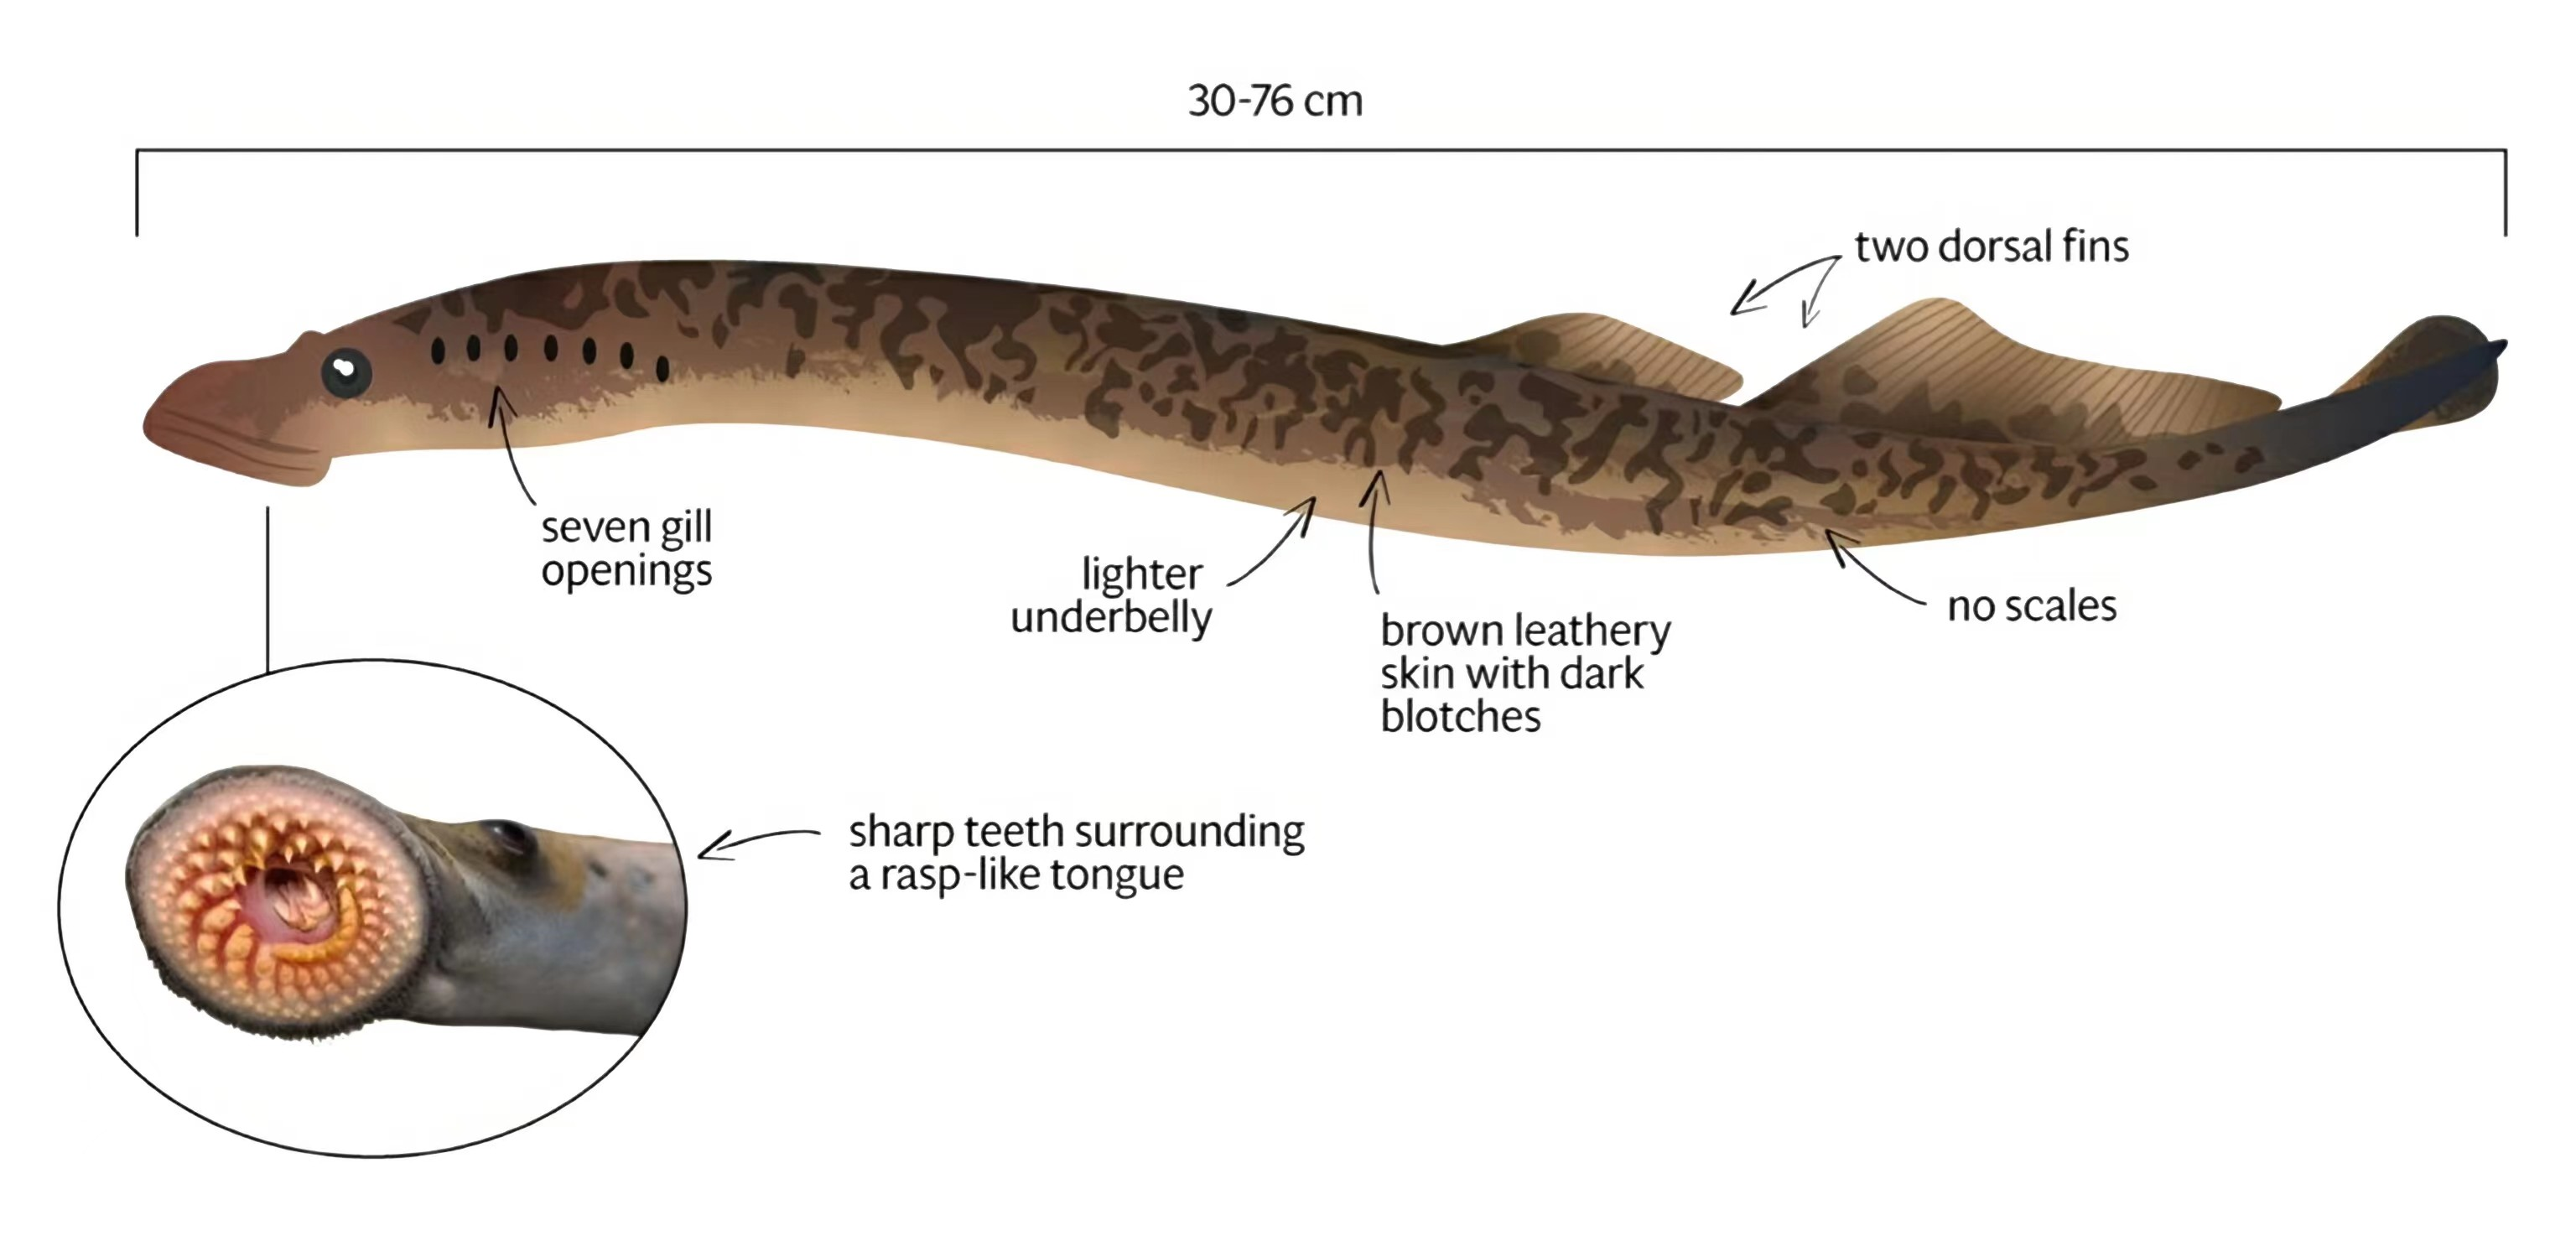
\includegraphics[width=15cm,height=10cm]{七鳃鳗生理结构示意图}
     \caption{Schematic diagram of the physiological structure of lampreys}
     \label{fig:Schematic diagram of the physiological structure of lampreys}
\end{figure}

The life cycle of the lamprey comprises several key stages, as shown in the figure\ref{fig:Illustration of the Life Cycle of the Lamprey}:

\begin{enumerate}
\item LARVA STAGE: The juvenile stage where they swim in the water with elongated and transparent bodies.
\item PARASITIC JUVENILE STAGE: Parasitic Juvenile stage where they infect and parasitize adult fish.
\item SPANNING NINETEEN ADULTS STAGE: The mature reproductive stage where they migrate to lakes to mate and spawn.
\item DOWNSTREAM MIGRATION TO LAKES STAGE: The adult stage where they migrate from the middle and lower reaches of rivers to lakes where they spend the winter in the blood of their host fish. 
\end{enumerate}

 These detailed information helps us to understand the ecological characteristics and life cycle of the sevengill eel more comprehensively, and is important for the study of the impact of its sex change on the ecological environment.
%七鳃鳗的身体细长如鳗鱼,没有真正的鳍,头部有圆形的吸盘状口盘,用于附着和吸血。身体两侧排列着七个呼吸孔,是其最显著的特征之一。七鳃鳗的生命周期包括在淡水溪流中繁殖、在海水中成长。成体通常在春季返回淡水溪流中繁殖,而幼虫则在河流中生活数年,之后迁移到海中继续成长。它们主要以滤食微生物和有机碎屑为食,成体有时会寄生在其他鱼类上。
%七鳃鳗的生命周期包括几个关键阶段:LARVA阶段:幼鱼期,它们在水中游动,身体细长且透明。PARASITIC JUVENILE阶段:寄生幼年阶段,它们会感染并寄生在成年鱼体内。SPANNING NINETEEN ADULTS阶段:成熟繁殖阶段,它们会迁移到湖泊中进行交配和产卵。DOWNSTREAM MIGRATION TO LAKES阶段:成鱼阶段,它们会从河流中下游迁移到湖泊中,并在那里以宿主鱼类的血液度过冬季。这些详细信息有助于我们更全面地了解七鳃鳗的生态特性和生命周期,对于研究其性别变化对生态环境的影响具有重要意义

\begin{figure}[htbp]
       \centering    
   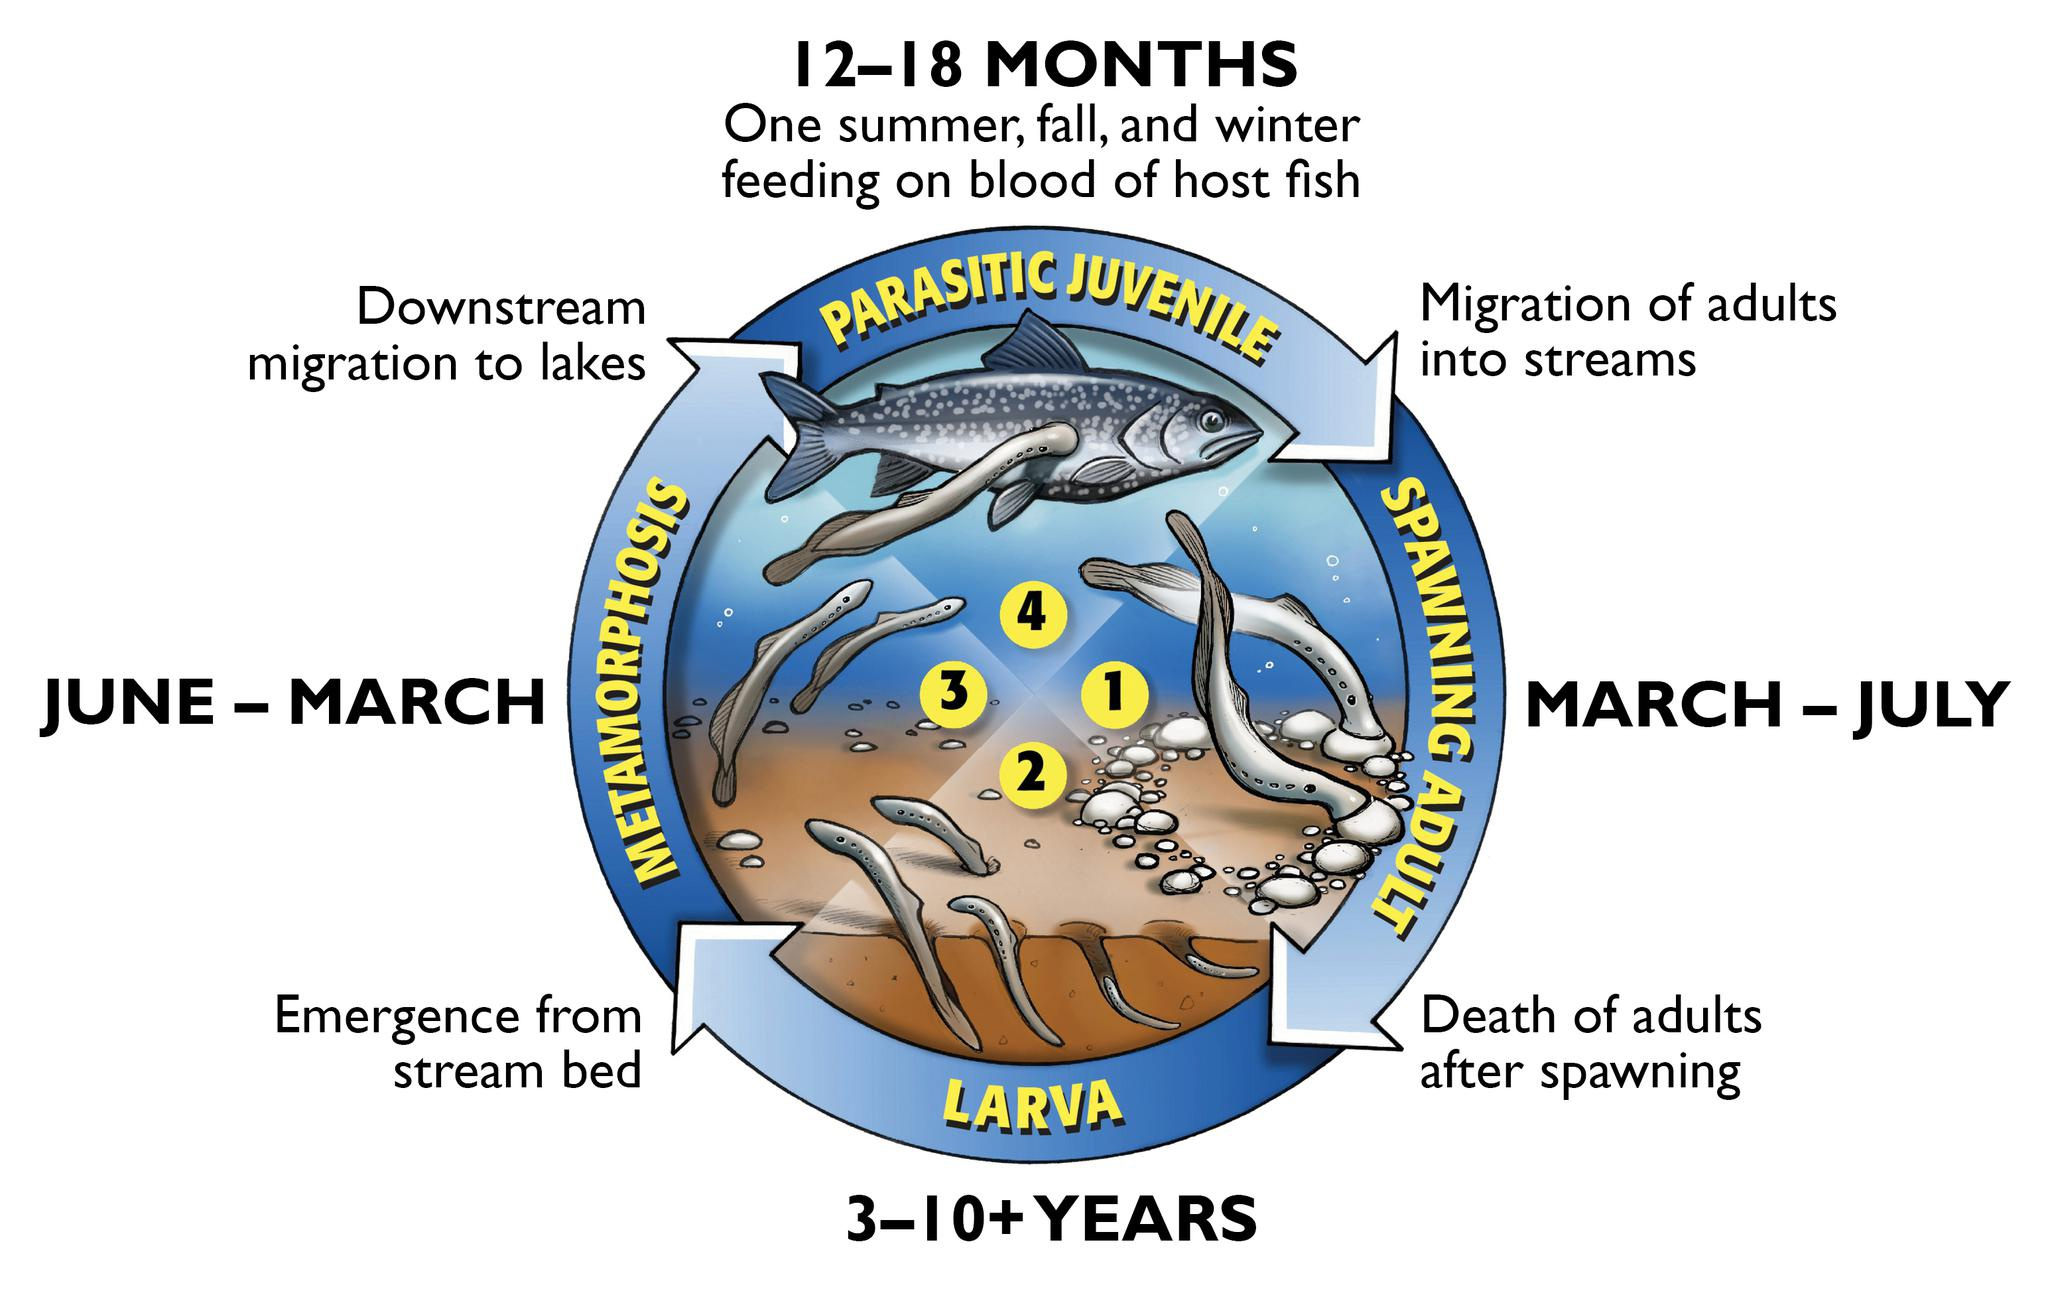
\includegraphics[width=15cm,height=10cm]{七鳃鳗的生长周期示意图}
     \caption{Illustration of the Life Cycle of the Lamprey}
     \label{fig:Illustration of the Life Cycle of the Lamprey}
\end{figure}

\subsubsection*{The impact of lampreys on ecology}
Investigations have revealed the significant impacts of the sea sevengill eel on the Great Lakes ecosystem of North America\cite{DangGuanchao2022}.In particular, the invasion of the sea lamprey into the North American Great Lakes has caused significant damage to fisheries production in the region. In addition, a case study conducted in the Cheboygan River in Michigan explored the larval and juvenile stages of the sevengill, their habitat preferences, and the control measures employed, such as sterile male release techniques. The study also discusses the various challenges faced in controlling sevengill populations due to habitat changes Together, these studies reveal the intricate relationship between the sea sevengill and the Great Lakes ecosystem\cite{JOHNSON2021S492}.
%通过调查,发现海七鳃鳗对北美五大湖生态系统的重大影响。特别是海七鳃鳗入侵北美五大湖,对该地区的渔业生产造成了重大损害。此外,在密歇根州的切博伊根河进行的一项案例研究探讨了七鳃鳗的幼虫和幼鱼阶段、它们的栖息地偏好以及所采取的控制措施,如不育雄性释放技术。该研究还讨论了由于栖息地变化而面临的控制七鳃鳗种群的各种挑战这些研究共同揭示了海七鳃鳗与五大湖生态系统之间错综复杂的关系。

Studies\cite{sex determination of lamprey} have revealed that the sex-determining mechanisms of sevengill sea lampreys are influenced by larval growth rates,as shown in the figure\ref{fig:The Impact of Lamprey Sex on the Ecological Environment}. Non-productive environments increasingly tend to produce more males, while productive environments increasingly do not tend to produce more males.Changes in the sex ratio of sevengill eels may have significant ecosystem impacts. For example, if an increase in the proportion of males leads to a decrease in reproduction rates, then the impact of the sevengill on its host fish may be reduced, thus affecting the food chain. In addition, changes in sex ratios may also affect the genetic diversity and adaptive capacity of sevengill eel populations. These suggest that the sex ratio of sevengill eels and its specific effects on ecosystems is a complex issue that requires further ecological modeling and research for a deeper understanding.
%研究表明,七鳃鳗的性别决定机制受到幼虫生长速度的影响。非生产性环境越来越倾向于产生更多雄性,而生产性环境则越来越不倾向于产生更多雄性。七鳃鳗性别比例的变化可能会对生态系统产生重大影响。例如,如果雄性比例增加导致繁殖率下降,那么七鳃鳗对其宿主鱼类的影响可能会减少,从而影响到食物链。此外,性别比例的变化也可能影响七鳃鳗种群的遗传多样性和适应能力。这些表明七鳃鳗的性别比例及其对生态系统的具体影响是一个复杂的问题,需要进一步的生态学模型和研究来深入理解。

\begin{figure}[htbp]
       \centering    
   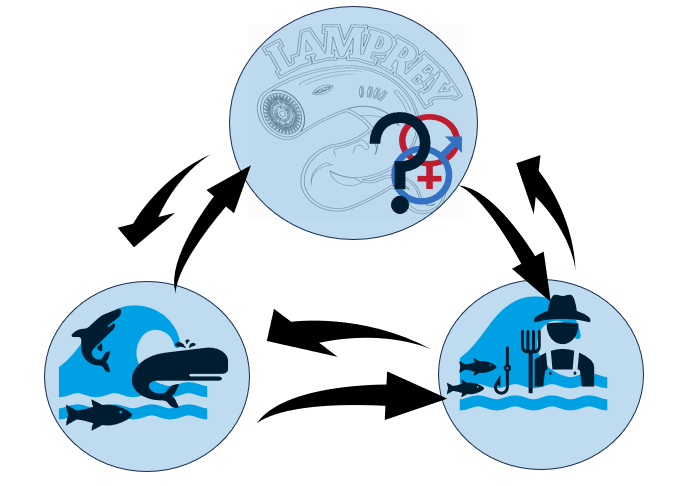
\includegraphics[width=15cm,height=10cm]{七鳃鳗性别对生态环境影响}
     \caption{The Impact of Lamprey Sex on the Ecological Environment}
     \label{fig:The Impact of Lamprey Sex on the Ecological Environment}
\end{figure}

\subsection{Research objective}
This study aimed to investigate the potential impacts of the sex ratio of sevengill eels on the ecosystem and to analyze their adaptive advantages and potential disadvantages under changes in resource availability. The team reveals the ecological impacts of sex ratio fluctuations by developing an ecological model to simulate how local environmental conditions affect the sex ratio of sevengill eels, especially their sex changes under different food availability conditions. The central question of this investigation is how the ability of sevengill populations to alter sex ratios affects the wider ecosystem, the benefits and drawbacks for the sevengill population itself, and the potential benefits that may accrue to other organisms within the ecosystem (e.g., parasites) that may shape the overall ecological equilibrium.
%本研究旨在探讨七鳃鳗性别比例对生态系统的潜在影响,并分析其在资源可获得性变化下的适应优势与潜在劣势。团队通过开发一个生态模型,模拟当地环境条件如何影响七鳃鳗的性别比例,特别是它们在不同食物供应条件下的性别变化,揭示性别比例波动对生态环境的影响。这项调查的核心问题是七鳃鳗种群改变性别比例的能力如何影响更广泛的生态系统,对七鳃鳗种群本身的利弊,以及可能对生态系统内其他生物(如寄生虫)产生的潜在益处,从而塑造整体的生态平衡。

\subsection{Our Work}
Our work encompasses a variety of mathematical models, including the Lotka-Volterra model, cellular automata model, and host-parasite dynamics model, to study the impact of the sex ratio change of lampreys on their ecological environment. We found that the change in sex ratio has adaptive advantages in improving predation efficiency and resisting parasites, but it also has potential negative impacts. Despite the limitations of the models in simulating complex environmental conditions and considering the impact of human activities, our research still provides important references for in-depth understanding of the impact of the sex ratio change of lampreys on their ecological environment.
%我们的工作涵盖了多种数学模型,包括Lotka-Volterra模型、元胞自动机模型和寄主-寄生虫动力学模型,用于研究七鳃鳗性别比例变化对其生态环境的影响。我们发现性别比例变化在提高捕食效率和抵抗寄生虫方面具有适应性优势,但同时也存在潜在的负面影响。尽管模型在模拟复杂环境条件和考虑人类活动影响方面存在局限性,我们的研究仍为深入理解七鳃鳗性别比例变化对生态环境的影响提供了重要参考。
\begin{figure}[htbp]
       \centering    
   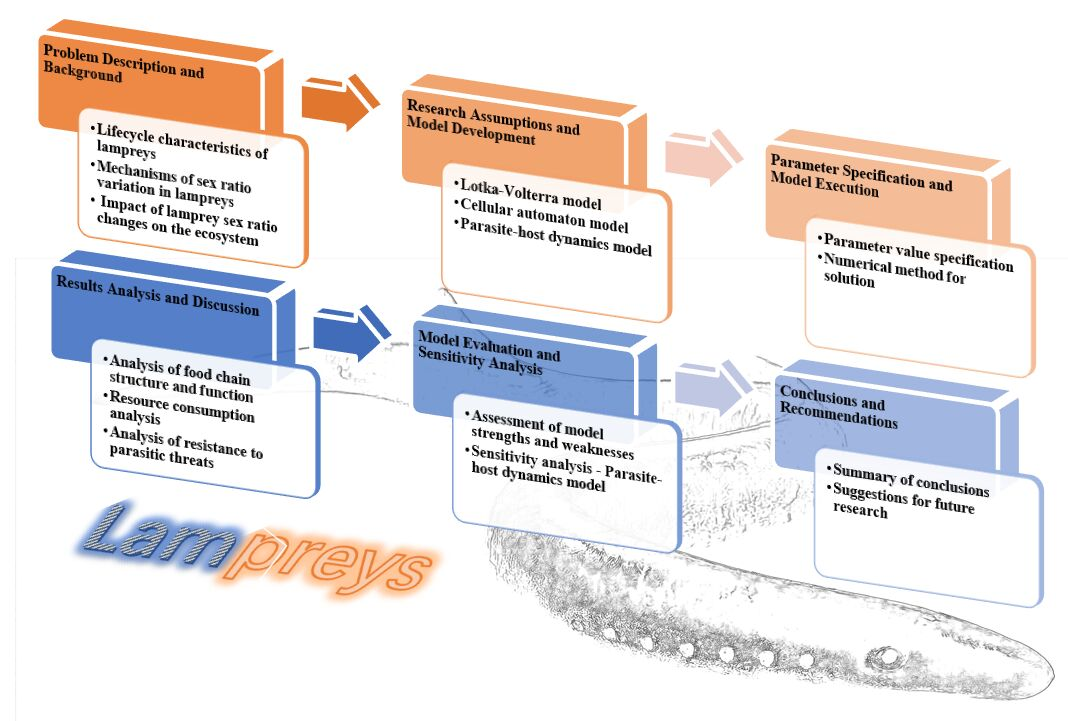
\includegraphics[width=15cm,height=10cm]{our work e}
     \caption{Our work for the Impact of Lamprey Sex on the Ecological Environment}
     \label{fig:Our work for the Impact of Lamprey Sex on the Ecological Environment}
\end{figure}

\section{Assumptions and Justificationsl}

Through a complete analysis of the problem, in order to simplify our model, we make the following reasonable assumptions.

\textbf{Assumption 1 : Assuming that environmental conditions remain constant throughout the course of the study.}
% 假设环境条件在研究期间保持不变。

% 静态环境提供了一个相对稳定的背景,使得我们能够更容易地追踪和分析性别比例的变化。
\textbf{Justification: }Static environments provide a relatively stable context that makes it easier to track and analyze changes in sex ratios.

\textbf{Assumption 2 : Assuming that the studied lamprey population is a closed system, without taking into account the influence of migration and movement.}
% 假设所研究的七鳃鳗是一个封闭的种群,不考虑移民和迁徙的影响。

% 在封闭种群的前提下,可以更准确地分析食物充足与否对种群内部性别比例的影响。
\textbf{Justification: }In the context of closed populations, the effect of food sufficiency on sex ratios within populations can be analyzed more accurately.

\textbf{Assumption 3 : Assuming that mating between individuals is random and the fixed mating ratio between males and females is maintained.}
% 假设个体之间的交配是随机的且雌雄交配比例固定。

% 假设个体之间的交配是随机的,有助于模拟自然繁殖过程,同时也简化了模型的复杂性,不会受到特定交配模式的干扰。
\textbf{Justification: }Assuming that mating between individuals is random helps to simulate the natural reproduction process and also simplifies the complexity of the model by not being disturbed by specific mating patterns.

\textbf{Assumption 4 :It is assumed that the survival rate of individuals, the mortality rate is known and does not vary with the sex ratio..}
% 假设个体的生存率,死亡率是已知的,并且不随着性别比的变化而变化。

%生存率和死亡率作为固定参数,可以理解为鳗鱼由于寿命衰老致死率,这类致死率往往不受其他因素影响。
\textbf{Justification: }Survival and mortality as fixed parameters can be interpreted as eel lethality due to longevity senescence, and such lethality is often unaffected by other factors.

\textbf{Assumption 5 :Assuming that changes in the sex ratio arise from interactions during the process of adapting to the ecological environment, with full consideration given to the impacts on ecosystem functions, on other species, and on the stability of the ecosystem.}
% 生态系统影响:假设性别比例的改变是来自于适应生态环境过程中的相互作用,充分考虑对生态系统功能的影响、对其他物种的影响和对生态系统稳定.

% 考虑到物种的种群特征是和基因和环境的相互作用下表现出来的,所以考虑对生态系统功能的影响、对其他物种的影响和对生态系统稳定是去研究七鳃鳗性别比例差异的必要条件。
\textbf{Justification: }Considering that a species’ population characteristics are expressed through the interaction of genes and the environment, it is necessary to examine the impacts on ecosystem functions, on other species, and on ecosystem stability in order to study the differences in sex ratio among lampreys.

\textbf{Assumption 6 :Considering the conditions for the LV (Lotka-Volterra) model to hold, we assume that the prey's growth is solely influenced by the predator. In the absence of predators, the prey can grow exponentially. The predator's functional response is linear, and in the absence of prey, the predator will decline exponentially.
}
% 考虑到LV模型的成立条件,假设食饵的增长仅受捕食者的影响,在没有捕食者的情况下,它可以以指数形式增长,捕食者的反应功能函数为线性的,没有食饵时,捕食者将以指数灭亡。

%为了简化捕食者-食饵相互作用的复杂性,便于数学处理和分析。这些假设使得模型能够单独研究捕食者对食饵种群的影响,并以指数形式描述种群增长和下降的趋势
\textbf{Justification: }To simplify the complexity of predator-prey interactions for ease of mathem\newpageal manipulation and analysis, these assumptions allow the model to isolate the effects of predators on prey populations and describe population growth and decline in exponential terms.

\newpage
\section{Notations}
The key mathematical notations used in this paper are listed in Table \label{Symbol Description}.
\begin{longtable}[hhhh]
  \centering
  \label{Symbol Description}
  \caption{Symbol Description}\\
  \begin{tabular}{cccc}
   \toprule
  Symbols & ~~~~~~~~~ & Meaning & ~~~~~~~~~\\
   \midrule
   $N_{1}$ & ~~~~~~~~~ & The population sizes of  a species & ~~~~~~~~~\\
   $K_{1}$  & ~~~~~~~~~ & The environmental carrying capacities for  a species & ~~~~~~~~~ \\
   $N_{2}$ & ~~~~~~~~~ & The population sizes of  a species & ~~~~~~~~~ \\
   $K_{2}$  & ~~~~~~~~~ & The environmental carrying capacities for  a species & ~~~~~~~~~\\
   $r_{1}$  & ~~~~~~~~~ & The population growth rates of  a species & ~~~~~~~~~ \\
   $P$  & ~~~~~~~~~ & The population that is preyed upon or parasitized & ~~~~~~~~~ \\
   $a$  & ~~~~~~~~~ & Capture rate of prey & ~~~~~~~~~ \\
  $S$  & ~~~~~~~~~ & Mortality rate & ~~~~~~~~~ \\
  $M$  & ~~~~~~~~~ &  The male population of lampreys & ~~~~~~~~~ \\
  $F$  & ~~~~~~~~~ &  The female population of lampreys & ~~~~~~~~~ \\
  $t$  & ~~~~~~~~~ &  Time & ~~~~~~~~~ \\
  $B$  & ~~~~~~~~~ & The birth rate & ~~~~~~~~~\\
  $N$  & ~~~~~~~~~ & The population sizes of lampreys & ~~~~~~~~~ \\
  $Z$  & ~~~~~~~~~ & The probability of transitioning to male & ~~~~~~~~~\\
  $S_{f}$  & ~~~~~~~~~ & The mortality rates of male lampreys & ~~~~~~~~~ \\
  $b_{f}$  & ~~~~~~~~~ & The predation efficiencies of female lampreys & ~~~~~~~~~ \\
  $S_{m}$  & ~~~~~~~~~ & The mortality rates of female lampreys & ~~~~~~~~~\\
  $b_{m}$  & ~~~~~~~~~ & The predation efficiencies of male lampreys & ~~~~~~~~~ \\
  $b$  & ~~~~~~~~~ & The proportion of males & ~~~~~~~~~ \\
  $c$  & ~~~~~~~~~ & Constant & ~~~~~~~~~ \\
  $\alpha$  & ~~~~~~~~~ & Constant & ~~~~~~~~~ \\
  $\beta$  & ~~~~~~~~~ & Constant & ~~~~~~~~~ \\
  $a_p$  & ~~~~~~~~~ & The probabilities of prey capture & ~~~~~~~~~ \\
  $a_a$  & ~~~~~~~~~ & The probabilities of lamprey capture & ~~~~~~~~~ \\
  $b_m$  & ~~~~~~~~~ & The capture capabilities of male lampreys & ~~~~~~~~~ \\
  $b_f$  & ~~~~~~~~~ & The capture capabilities of female lampreys& ~~~~~~~~~ \\
  $b_a$  & ~~~~~~~~~ & The capture capabilities of humans & ~~~~~~~~~ \\
  $A$  & ~~~~~~~~~ & The human population & ~~~~~~~~~ \\
   \bottomrule
\end{tabular}
\end{longtable}

\section{Analysis and Modeling}
%\subsection{Model Establishment and Solution for Question One}
\subsection{Model 1: Lotka–Volterra model}
% To investigate the impact of a particular trait of a species on the interactions and influences within and between populations, between species, and with the ecosystem, it is essential to grasp both the holistic and partial perspectives. This implies that we need to consider the issue from multiple levels and angles to comprehensively understand and describe the impact of species traits on ecosystems.

% Firstly, we must consider the impact of species traits on intrapopulation dynamics. Interactions among individuals within a population, such as competition, cooperation, and reproduction, may be influenced by species traits. For instance, traits such as reproductive strategies, life habits, and behavioral patterns could affect population growth rates, density dependence, and genetic diversity.

% Secondly, we need to examine the influence of species traits on interspecies interactions. Interactions between species, such as predation, symbiosis, and competition, are crucial drivers in ecosystems. Species traits may affect the relative advantages, interdependence, and stability of symbiotic relationships between species.

% Furthermore, we must also consider the impact of species traits on the ecosystem. Traits of a species may influence the structure, function, and stability of the ecosystem. For example, traits such as ecological niche, biogeographical distribution, and ecological adaptability could affect ecosystem species diversity, energy flow, and material cycling.

%为了研究一个物种的某个特性对种群间、与物种之间和与生态系统之间的相互作用和影响,我们必须要把握好整体联系和部分联系的视角。这意味着我们需要从多个层面和角度来考虑问题,以便全面地理解和描述物种特性对生态系统的影响。
%首先,我们需要考虑物种特性对种群内部的影响。种群内部个体间的相互作用,如竞争、合作、繁殖等,都可能受到物种特性的影响。例如,物种的繁殖策略、生活习性、行为模式等特性都可能影响种群的增长率、密度依赖性、遗传多样性等。
%其次,我们需要考虑物种特性对物种间相互作用的影响。物种间的相互作用,如捕食、共生、竞争等,是生态系统中重要的驱动因素。物种特性可能影响物种间的相对优势、相互依赖程度、共生关系的稳定性等。
%此外,我们还需要考虑物种特性对生态系统的影响。物种特性可能影响生态系统的结构、功能和稳定性。例如,物种的生态位、生物地理分布、生态适应性等特性都可能影响生态系统的物种多样性、能量流动、物质循环等。
\subsubsection{Description of Lotka–Volterra}
To comprehensively study the multifaceted impacts of species traits on ecosystems, we need to adopt interdisciplinary methods and tools. For instance, mathematical models can be used to simulate the effects of changes in species traits on population dynamics and ecosystem functioning.

In this regard, the Lotka-Volterra (LV) model is an excellent choice. The LV model, also known as the Predator-Prey model, is a classic ecological model used to describe the dynamic relationship in predator-prey systems. This model utilizes two nonlinear differential equations to describe the changes in predator and prey populations over time, thereby helping us to understand and predict the impact of species traits on ecosystems.\AIcite{AI3}

Firstly, the LV model can effectively describe the impact of species traits on intrapopulation dynamics. By adjusting model parameters, we can simulate the effects of lamprey traits such as reproductive strategies, life habits, and behavioral patterns on population growth, density dependence, and genetic diversity. For example, by setting parameters for changes in the sex ratio of lampreys, we can explore the impact of population sex ratios at different stages on internal dynamics, including competition, mating, and cooperation among male and female lampreys.

Secondly, the LV model can also effectively describe the influence of species traits on interspecies interactions. By adjusting model parameters, we can simulate how lamprey traits affect the relative advantages and interdependence in food chain relationships. Especially for lampreys, which are parasitic or semi-parasitic (feeding on organic matter), the LV model can analogously simulate this special level in the food chain and reveal the impact of lamprey population sex ratios on other species.

Additionally, the LV model can help us study the impact of species traits on ecosystems. By simulating changes in lamprey traits, we can observe changes in ecosystem structure, function, and stability. For example, by altering parameters related to the ecological niche of lampreys, we can investigate the impact of lamprey traits on ecosystem diversity and the flow of energy and material cycling within the ecosystem.

%为了全面地研究物种特性对生态系统的多方面影响,我们需要采用多学科的方法和手段。例如,我们可以利用数学模型来模拟物种特性的变化对种群动态和生态系统的影响。
%为此,LV模型是可以很好的选择。LV模型,即Lotka-Volterra模型,是一种经典的生态学模型,用于描述捕食者-猎物系统中的动态关系。该模型通过两个非线性微分方程来描述捕食者和猎物种群随时间的变化,从而帮助我们理解和预测物种特性对生态系统的影响。
%首先,LV模型可以很好地描述物种特性对种群内部的影响。通过调整模型参数,我们可以模拟七鳃鳗的繁殖策略、生活习性、行为模式等特性对种群增长、密度依赖性和遗传多样性的影响。例如,通过设置七鳃鳗的性别比例变化的参数,可以探究不同时期下种群的性别比例对其内部的影响,包括雌雄七鳃鳗之间大的竞争、交配、合作等。
%其次,LV模型也可以很好地描述物种特性对物种间相互作用的影响。通过调整模型参数,我们可以模拟七鳃鳗特性对食物链关系的相对优势和相互依赖程度的影响。尤其是七鳃鳗这种营寄生或者半寄生生活(以有机物为食),LV模型能够类比模拟出七鳃鳗这种特殊的食物链层次,并且揭示出七鳃鳗种群的性别比例对其他物种的影响。
%此外,LV模型还可以帮助我们研究物种特性对生态系统的影响。通过模拟七鳃鳗特性的变化,我们可以观察生态系统的结构、功能和稳定性等方面的变化。例如,通过改变七鳃鳗的生态位参数,我们可以研究七鳃鳗特性对生态系统多样性的影响和生态系统能量流动和物质循环的影响。


Firstly, it is important to understand that the Lotka-Volterra model (Lotka-Volterra interspecific competition model) is an extension of the logistic model (logistic growth model). According to the logistic model, the following relationship holds:
%首先,我们需要知道的是Lotka-Volterra模型(Lotka-Volterra种间竞争模型)是logistic模型(阻滞增长模型)的延伸。依logistic模型有如下关系:

\begin{equation}
\begin{aligned}
\frac{\mathrm{d} N_{1}}{\mathrm{d} t} = r_{1}\cdot N_{1}\cdot(1-\frac{N_{1}}{K_{1}})
\end{aligned}
\end{equation}

Where $N_{1}$ represent the population sizes of  a species, $K_{1}$ represent the environmental carrying capacities for  a species, $r_{1}$ represent the population growth rates of  a species, and $N/K$ can be understood as the proportion of space already utilized.
%其中,$N_{1}$:分别为物种的种群数量,$K_{1}$:分别为物种的环境容纳量,$r_{1}$:分别为物种的种群增长率,其中:$N/K$可以理解为已经利用的空间。

Essentially, the LV model takes into account the competition from other species and then extends the concept of available space as follows:
%本质上,LV模型考虑到来自其他的竞争关系,然后对未利用的空间进行一个扩展:

\begin{equation}
\begin{aligned}
\frac{\mathrm{d} N_{1}}{\mathrm{d} t} = r_{1}\cdot N_{1}\cdot(1-\frac{N_{1}}{K_{1}}-\frac{N_{2}}{K_{2}})
\end{aligned}
\end{equation}

\subsubsection{Semi-parasitic predator-prey model}
Returning to the context of the lamprey, our research team conducted a thorough investigation into its biological characteristics. Considering that lampreys are parasitic or semi-parasitic and their sex ratio can be altered by genetic and environmental pressures, we propose a semi-parasitic predator-prey model based on the fundamental LV model.
%回到七鳃鳗背景下的模型构建,我们研究团队在充分调查和研究其生物特点。考虑到七鳃鳗是一种营寄生或半寄生、性别比例受基因和环境压力可改变的物种,我们在最基本的LV模型上提出一种半寄生的捕食者-被捕食者模型。

Firstly, based on numerous relevant literature, we know that the food source of lampreys is plankton in the water or soil, and of course, some species of lampreys obtain resources by parasitizing on other fish. For the population P that is preyed upon or parasitized:
%第一点,根据以往诸多相关文献,我们可以知道七鳃鳗的食物来源是水中或者泥土里面的浮游生物,当然部分的七鳃鳗品种是会通过寄生在其他鱼类的身上获取资源。针对被捕食或寄生的种群P:

\begin{equation}
\begin{aligned}
\frac{\mathrm{d} P}{\mathrm{d} t} = r_{p}\cdot P-a \cdot P\cdot N
\end{aligned}
\end{equation}

Where $r_{p}$ represents the birth rate of the prey or parasitized population, $a$ represents the probability of being preyed upon or parasitized, and $N$ denotes the total number of lampreys in the population.
%其中$r_{p}$是被捕食或寄生的种群的出生率,$\alpha$是被捕食的概率,$N$表示七鳃鳗整个种群的数目。

Secondly, the varying sex ratio of lampreys with population changes requires careful consideration. Through literature review, it is observed that during the nesting stage, females are in the majority, but males become dominant during the spawning period. After spawning, females again become the majority. This suggests that the mating system of lampreys may be polygynous, with males reproducing in multiple nests, while females tend to spawn in the same nest. However, since lampreys are oviparous and can lay thousands of eggs at once, the impact of polygynous mating can be essentially ignored. At the same time, when lampreys spawn, some eggs may fall outside of the nest, facing the risk of death. In addition to this, differences in predation efficiency due to sexual differences can also lead to changes in the population. In summary, we can derive the population change equations for male lampreys M and female lampreys F as follows:
%第二点,针对七鳃鳗这种随种群变化而变化的性别比例需要我们谨慎考虑。通过查询资料:在筑巢阶段,雌性占主导地位,但在产卵期,雄性占优势。产卵后,雌性再次成为多数。这表明七鳃鳗的交配系统可能是一夫多妻制,雄性会在多个巢穴中繁殖,而雌性则倾向于在同一个巢穴中产卵。但是,由于七鳃鳗是卵生动物,一次性可产成千上万的鱼卵,所有可以基本忽略一夫多妻制交配的影响。同时,当七鳃鳗在产卵时部分卵会散落在巢穴外面,这时候就面临着死亡的风险。除此之外,性别差异所带来的捕食效率差异也会导致种群的变化。综上所述,我们可以得到雄性七鳃鳗M和雌性七鳃鳗F的种群变化方程:

\begin{equation}
\label{eq:MF}
\begin{aligned}
\frac{\mathrm{d} F}{\mathrm{d} t} &= B\cdot N\cdot (1-Z)-S_{f}\cdot F+b_{f}\cdot a \cdot P \cdot F \\
\frac{\mathrm{d} M}{\mathrm{d} t} &= B\cdot N\cdot Z-S_{m}\cdot M+b_{m}\cdot a \cdot P \cdot M
\end{aligned}
\end{equation}

Where $B$ represents the birth rate, $Z$ represents the probability of transitioning to male, $S_{f}$ and $S_{m}$ are the mortality rates of female and male lampreys, respectively, and $b_{f}$ and $b_{m}$ are the predation efficiencies of female and male lampreys, respectively.
%其中,$B$是出生率,$Z$是转变雄性的概率,$S_{f}$和$S_{m}$分别是雌雄七鳃鳗的死亡率,$b_{f}$和$b_{m}$分别是雌雄七鳃鳗的捕食效率。

Thirdly, considering the birth rate and taking into account the tendency of lampreys towards polygyny, we can obtain the birth rate \( B \) as follows:
%第三点,针对出生率,充分考虑到七鳃鳗种群的一夫多妻制的倾向性,我们可以得到出生率B:

\begin{equation}
\begin{aligned}
B=b\cdot (1-b)\cdot c
\end{aligned}
\end{equation}

Where $c$ is a constant and $b$ represents the proportion of males, calculated as $\frac{M}{M+F}$.
%其中$c$是常数,$b$为雄性占比,即$\frac{M}{M+F}$。

Fourthly, regarding the sex transformation of lampreys, according to the data, lampreys are sexually undifferentiated in their juvenile stage, with their gonads not yet developed, and they do not distinguish between male and female until they are influenced by environmental pressures and gene expression, at which point they begin to differentiate sex. Therefore, we use the following function for fitting, with the unknowns being parameters:
%第四点,针对七鳃鱼的性别转变,根据资料,七鳃鱼在幼年时期的性腺未发育完成,不分雌雄,直到收到环境压力和基因的表达,在开始分化性别。故我们采用以下函数进行拟合,其中未知数均为参数:

\begin{equation}
\begin{aligned}
Z_{M}=\frac{\gamma }{1+p^{\alpha } } +\beta 
\end{aligned}
\end{equation}
\subsubsection{Tri-trophic model}
Based on numerous relevant literature studies, we know that the lamprey serves as a food source in certain regions of the world. In considering the impact of human predation on lampreys, we introduce their predators into a Semi-parasitic predator-prey model, creating a three-tiered model. This three-tiered model helps reveal the cascading effects of human predation on other species, particularly the impact on predators that depend on lampreys. Additionally, the adoption of a three-tiered trophic model can provide effective strategies for resource management, balancing human needs with ecological conservation. In terms of conservation efforts, this model can predict the effects of human predation on lampreys and other species, offering guidance for maintaining biodiversity and ecological balance. In summary, the three-tiered trophic model provides a crucial tool for comprehensively understanding the impact of human predation activities on ecosystems.

%根据以往诸多相关文献,我们知道七鳃鳗作为世界某些地区的食物来源。所以我们考虑人类捕食对七鳃鳗的影响,我们在Semi-parasitic predator-prey model基础对七鳃鳗引入其捕食者,构成三级模型。三级模型有助于揭示人类捕食对其他物种的级联效应,尤其是对依赖七鳃鳗的捕食者的影响。此外,采用三级营养模型可以为资源管理提供有效的策略,平衡人类需求与生态保护。对于保护工作,该模型可以预测人类捕食对七鳃鳗及其他物种的影响,为维护生物多样性和生态平衡提供指导。综上所述,三级营养模型为全面理解人类捕食活动对生态系统的影响提供了关键的工具。

% 我们在\ref{eq:MF}的基础上加上人类这个捕食者对七鳃鳗的影响,其中$a_p$,$a_a$为猎物被捕获的概率与七鳃鳗被捕获的概率。$b_m$, $b_f$,$b_a$为雄七鳃鳗,雌七鳃鳗,人类的捕获能力,$A$为人类的数量,因此对于七鳃鳗有以下方程。
On the basis of Equation \ref{eq:MF}, we incorporate the impact of humans as predators on lampreys, where $a_p$ and $a_a$ represent the probabilities of prey and lamprey capture, respectively. $b_m$, $b_f$, and $b_a$ denote the capture capabilities of male lampreys, female lampreys, and humans, while $A$ represents the human population. Therefore, for lampreys, the following equations hold.
\begin{equation}
\begin{aligned}
\frac{\mathrm{d} F}{\mathrm{d} t} &= B\cdot N\cdot (1-Z)-S_{f}\cdot F+b_{f}\cdot a_p \cdot P \cdot F - a_a \cdot b_a \cdot A \cdot F \\
\frac{\mathrm{d} M}{\mathrm{d} t} &= B\cdot N\cdot Z-S_{m}\cdot M+b_{m}\cdot a \cdot P \cdot M - a_a \cdot b_a \cdot A \cdot M
\end{aligned}
\end{equation}
%对于人类,假设$d_a$为人类在无七鳃鳗时候的死亡率,因此有以下方程。
\begin{equation}
\begin{aligned}
dA = - d_a \cdot A + b_a \cdot a_a \cdot A \cdot N
\end{aligned}
\end{equation}

\subsubsection{Result}
For the above system of differential equations, we employ the fourth-order Runge-Kutta method for numerical solution. This method approximates the solution of a differential equation through calculations at four intermediate steps. For a given first-order ordinary differential equation of the form:
\[ \frac{dy}{dt} = f(t, y) \]
where \(y\) is the unknown function, \(t\) is the independent variable, and \(f(t, y)\) describes the function governing the change of \(y\) with respect to time \(t\). Using the fourth-order Runge-Kutta method, the solution at the next time step \(y_{n+1}\) can be obtained as follows:
% 对于上面的微分方程模型我们使用四阶龙格库塔求解。它通过四个中间步骤的计算来逼近微分方程的解。这个方法相对简单而又相当精确。
% 对于给定一个一阶常微分方程:
% \[ \frac{dy}{dt} = f(t, y) \]
% 其中 \(y\) 是未知函数,\(t\) 是自变量,而 \(f(t, y)\) 是描述 \(y\) 随时间 \(t\) 变化的函数。使用四阶龙格库塔方法,下一个时间步的解 \(y_{n+1}\) 可以如此得到:
\begin{equation}
\begin{aligned}
k_1 &= f(t_n, y_n) \\
k_2 &= f(t_n + \frac{h}{2}, y_n + \frac{h}{2}k_1) \\
k_3 &= f(t_n + \frac{h}{2}, y_n + \frac{h}{2}k_2) \\
k_4 &= f(t_n + h, y_n + hk_3) \\
y_{n+1} &= y_n + \frac{h}{6}(k_1 + 2k_2 + 2k_3 + k_4) \\
\end{aligned}
\end{equation}
% 其中,tn 是当前时间,yn 是当前解,h 是时间步长。
In this context, \(t_n\) represents the current time, \(y_n\) is the current solution, and \(h\) denotes the time step size.
 % c = 0.08 #生殖率
 %    k = 0.01 #控制性转率
 %    N = M + F # 总数
 %    b = M / N #雄占比
 %    B = b * (1 - b) * c # 繁殖率
 %    Z = 0.30 / (2 + y[2]**k) + 0.53 #转雄概率
 %    rp, da = 0.09, 0.004# P生存率, a死亡率
 %    dm, df = 0.045, 0.035 #死亡率
 %    bm, bf, ba = 0.5, 0.4, 0.05 #捕获能力
 %    ap, aa = 0.002, 0.002#被捕率
\begin{table}[htbp]
  \centering
  \label{Parameter Settings1}
  \caption{Parameter Settings1}
  \begin{tabular}{cccc}
   \toprule
    Parameter name & Parameter value & Parameter name & Parameter value\\
    \midrule
    $c$ & 0.08 & $d_f$ & 0.035\\
    \alpha & 0.01 & $b_m$ & 0.5 \\
    \beta & 0.53 & $b_f$ & 0.4 \\
    $r_p$ & 0.09 & $b_a$ & 0.05 \\
    $d_a$ & 0.004 & $a_p$ & 0.002 \\
    $d_m$ & 0.045 & $a_a$ & 0.002\\   
  \bottomrule
\end{tabular}
\end{table}

By setting the parameters as outlined in the table\ref{Parameter Settings1} and employing the fourth-order Runge-Kutta method for computation, we have generated a simulation graph depicting the dynamics of time, prey, seven-gilled sharks (Hexanchus griseus), and humans. As illustrated in Figure \ref{fig:population_model_simulation}, we observe that over time, the increasing population of seven-gilled sharks necessitates a higher consumption of prey, leading to a gradual decline in prey numbers. This trend continues until prey becomes exceptionally scarce, triggering a state of hunger in the seven-gilled sharks and causing a sharp decline in their population. At this point, some prey manages to survive, initiating a resurgence in prey numbers. The alternating increase and decrease in the populations of prey and seven-gilled sharks establish a dynamic equilibrium within the ecosystem.

Simultaneously, humans rely on seven-gilled sharks as a food source. With the rise in the seven-gilled shark population, human numbers also increase. However, as the availability of seven-gilled shark food decreases, human numbers decrease as well. Due to humans not solely depending on seven-gilled sharks for sustenance and the gradual advancement of human society, the human population exhibits a trend of continuous growth.
% 通过设定如表的参数,通过四阶龙格库塔的计算,我们得到时间-猎物-七鳃鳗-人类图。如图\ref{population_model_simulation}所示,我们看到随着时间变化,由于七鳃鳗数量的增多而需要食用更多的猎物,此时猎物的数量正在下降,直到猎物数量特别少时,七鳃鳗进入了饥饿的状态而使得七鳃鳗的数量急剧下降,这时部分猎物得以存活,猎物数量重新开始回升;猎物与七鳃鳗的数量交替增减形成了生物圈中的动态平衡。同时人类以七鳃鳗为食会随着七鳃鳗上升也增加,随着食物七鳃鳗减少而减少,由于人类不仅以七鳃鳗为食,和人类发展水平逐渐提升,人类的数量呈增加的趋势。

\begin{figure}[htbp]
       \centering    
   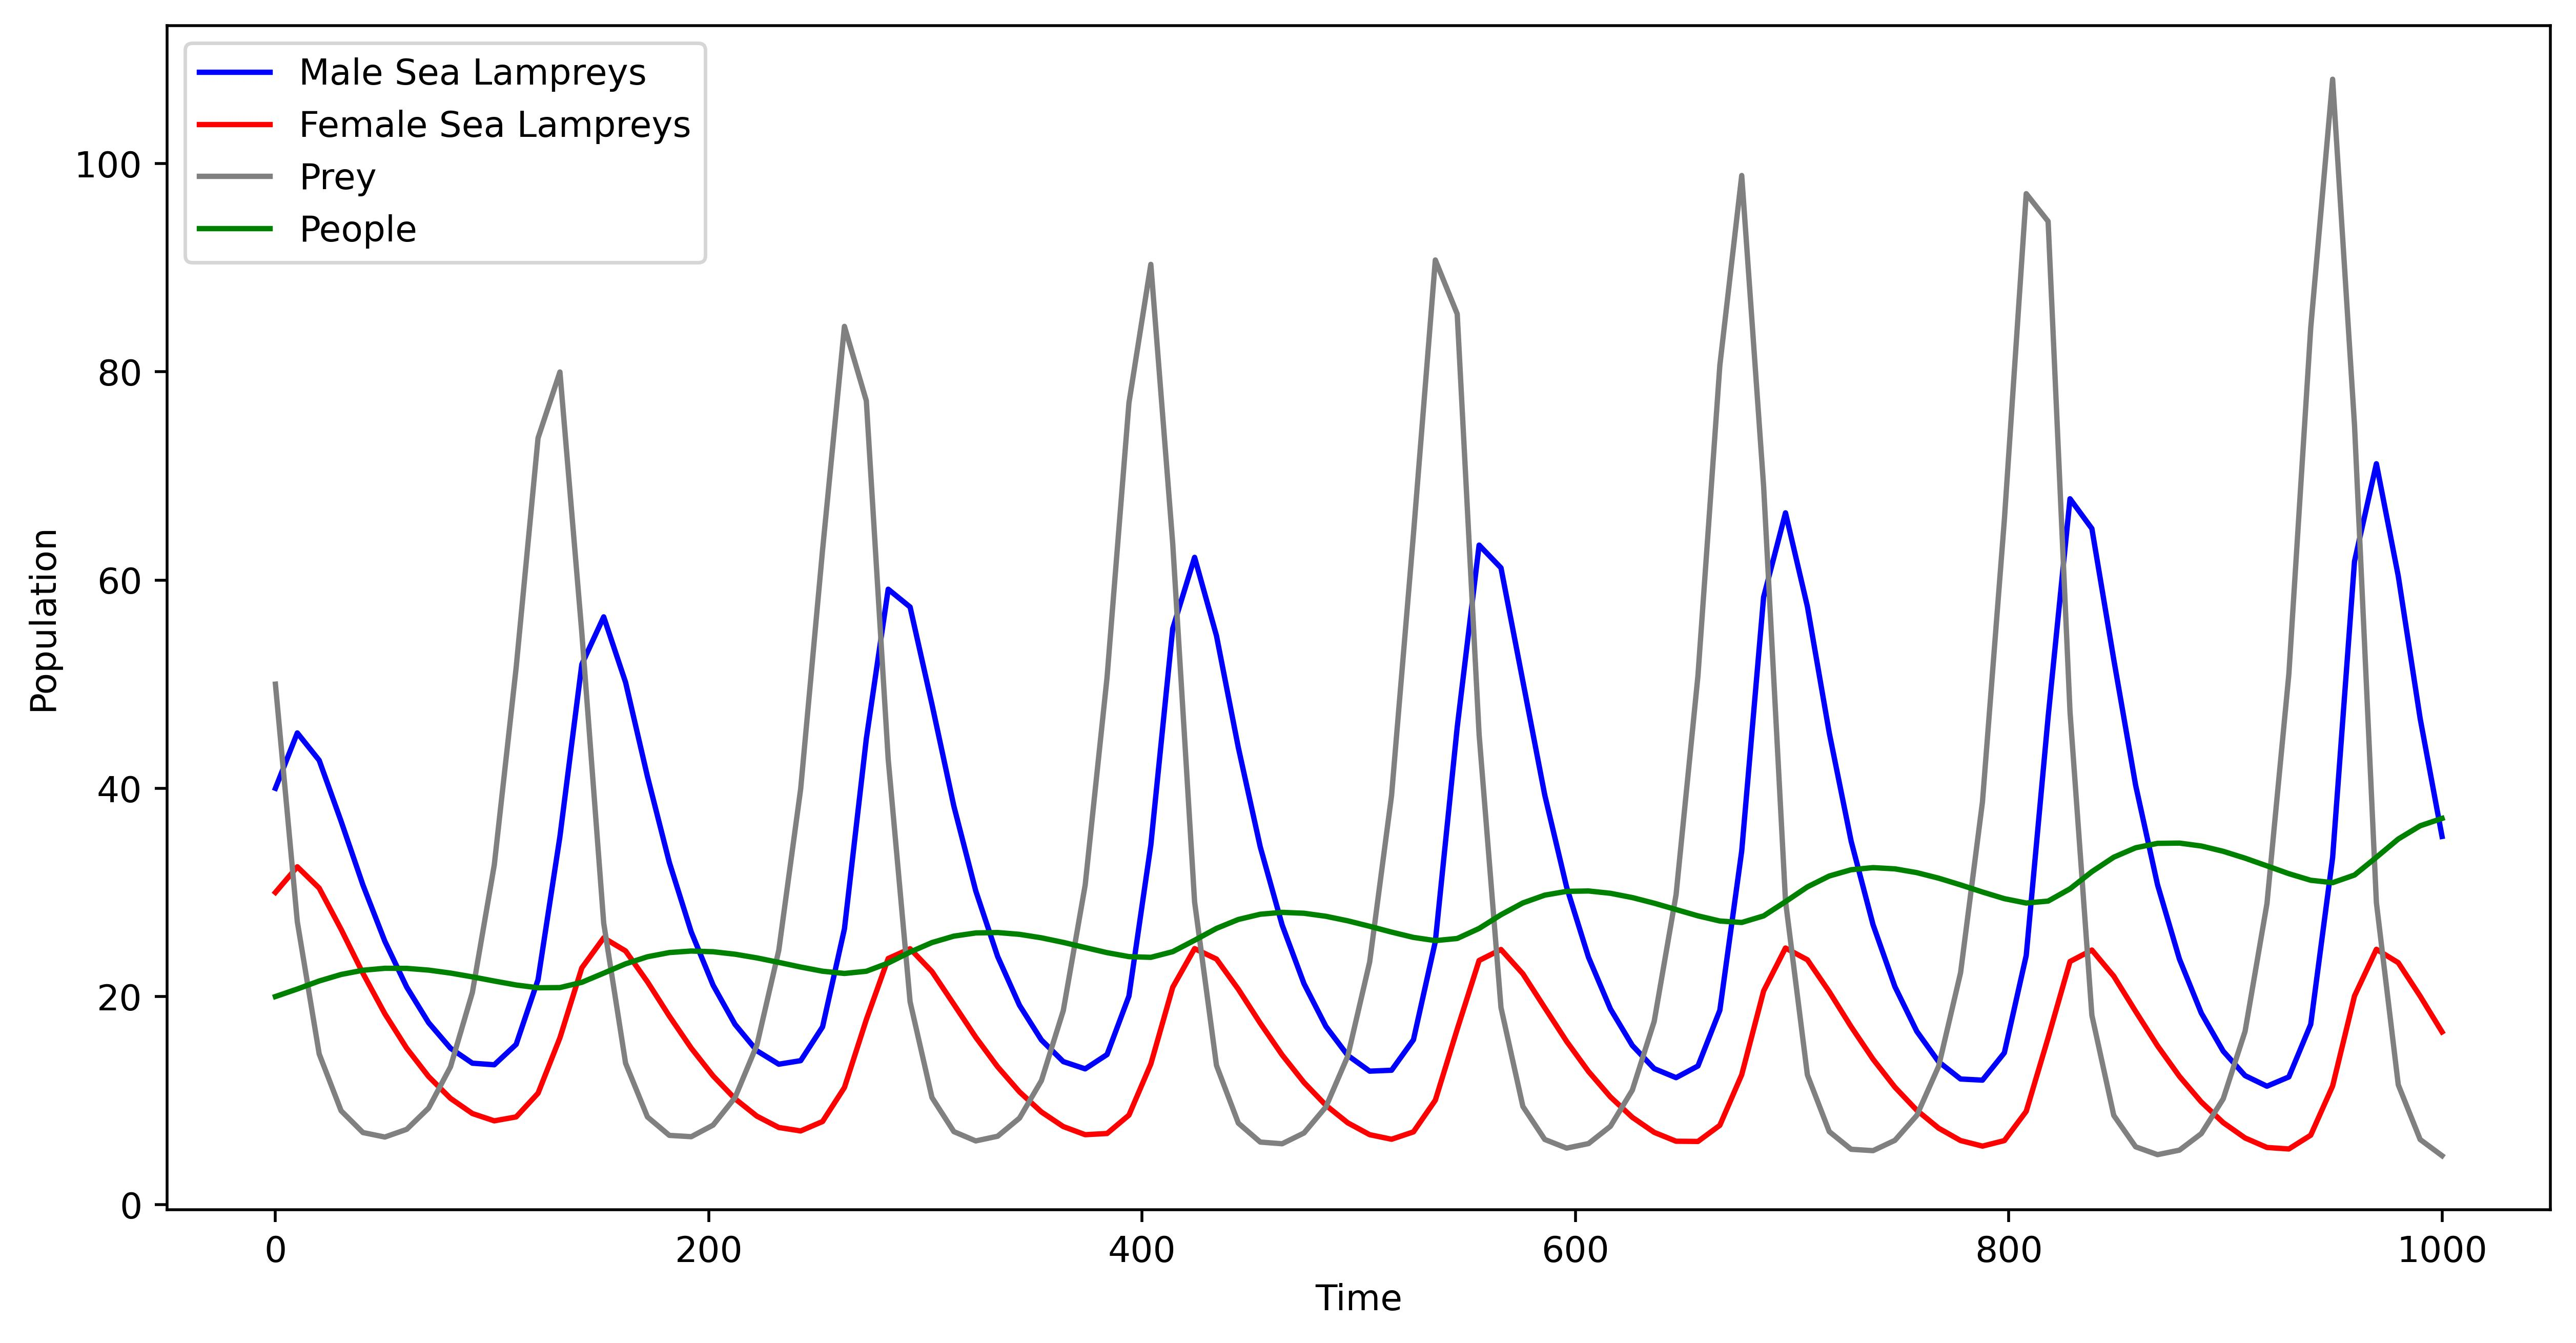
\includegraphics[width=15cm,height=9cm]{population_model_simulation}
     \caption{population\_model\_simulation}
     \label{fig:population_model_simulation}
\end{figure}

\begin{figure}[htbp]
       \centering    
   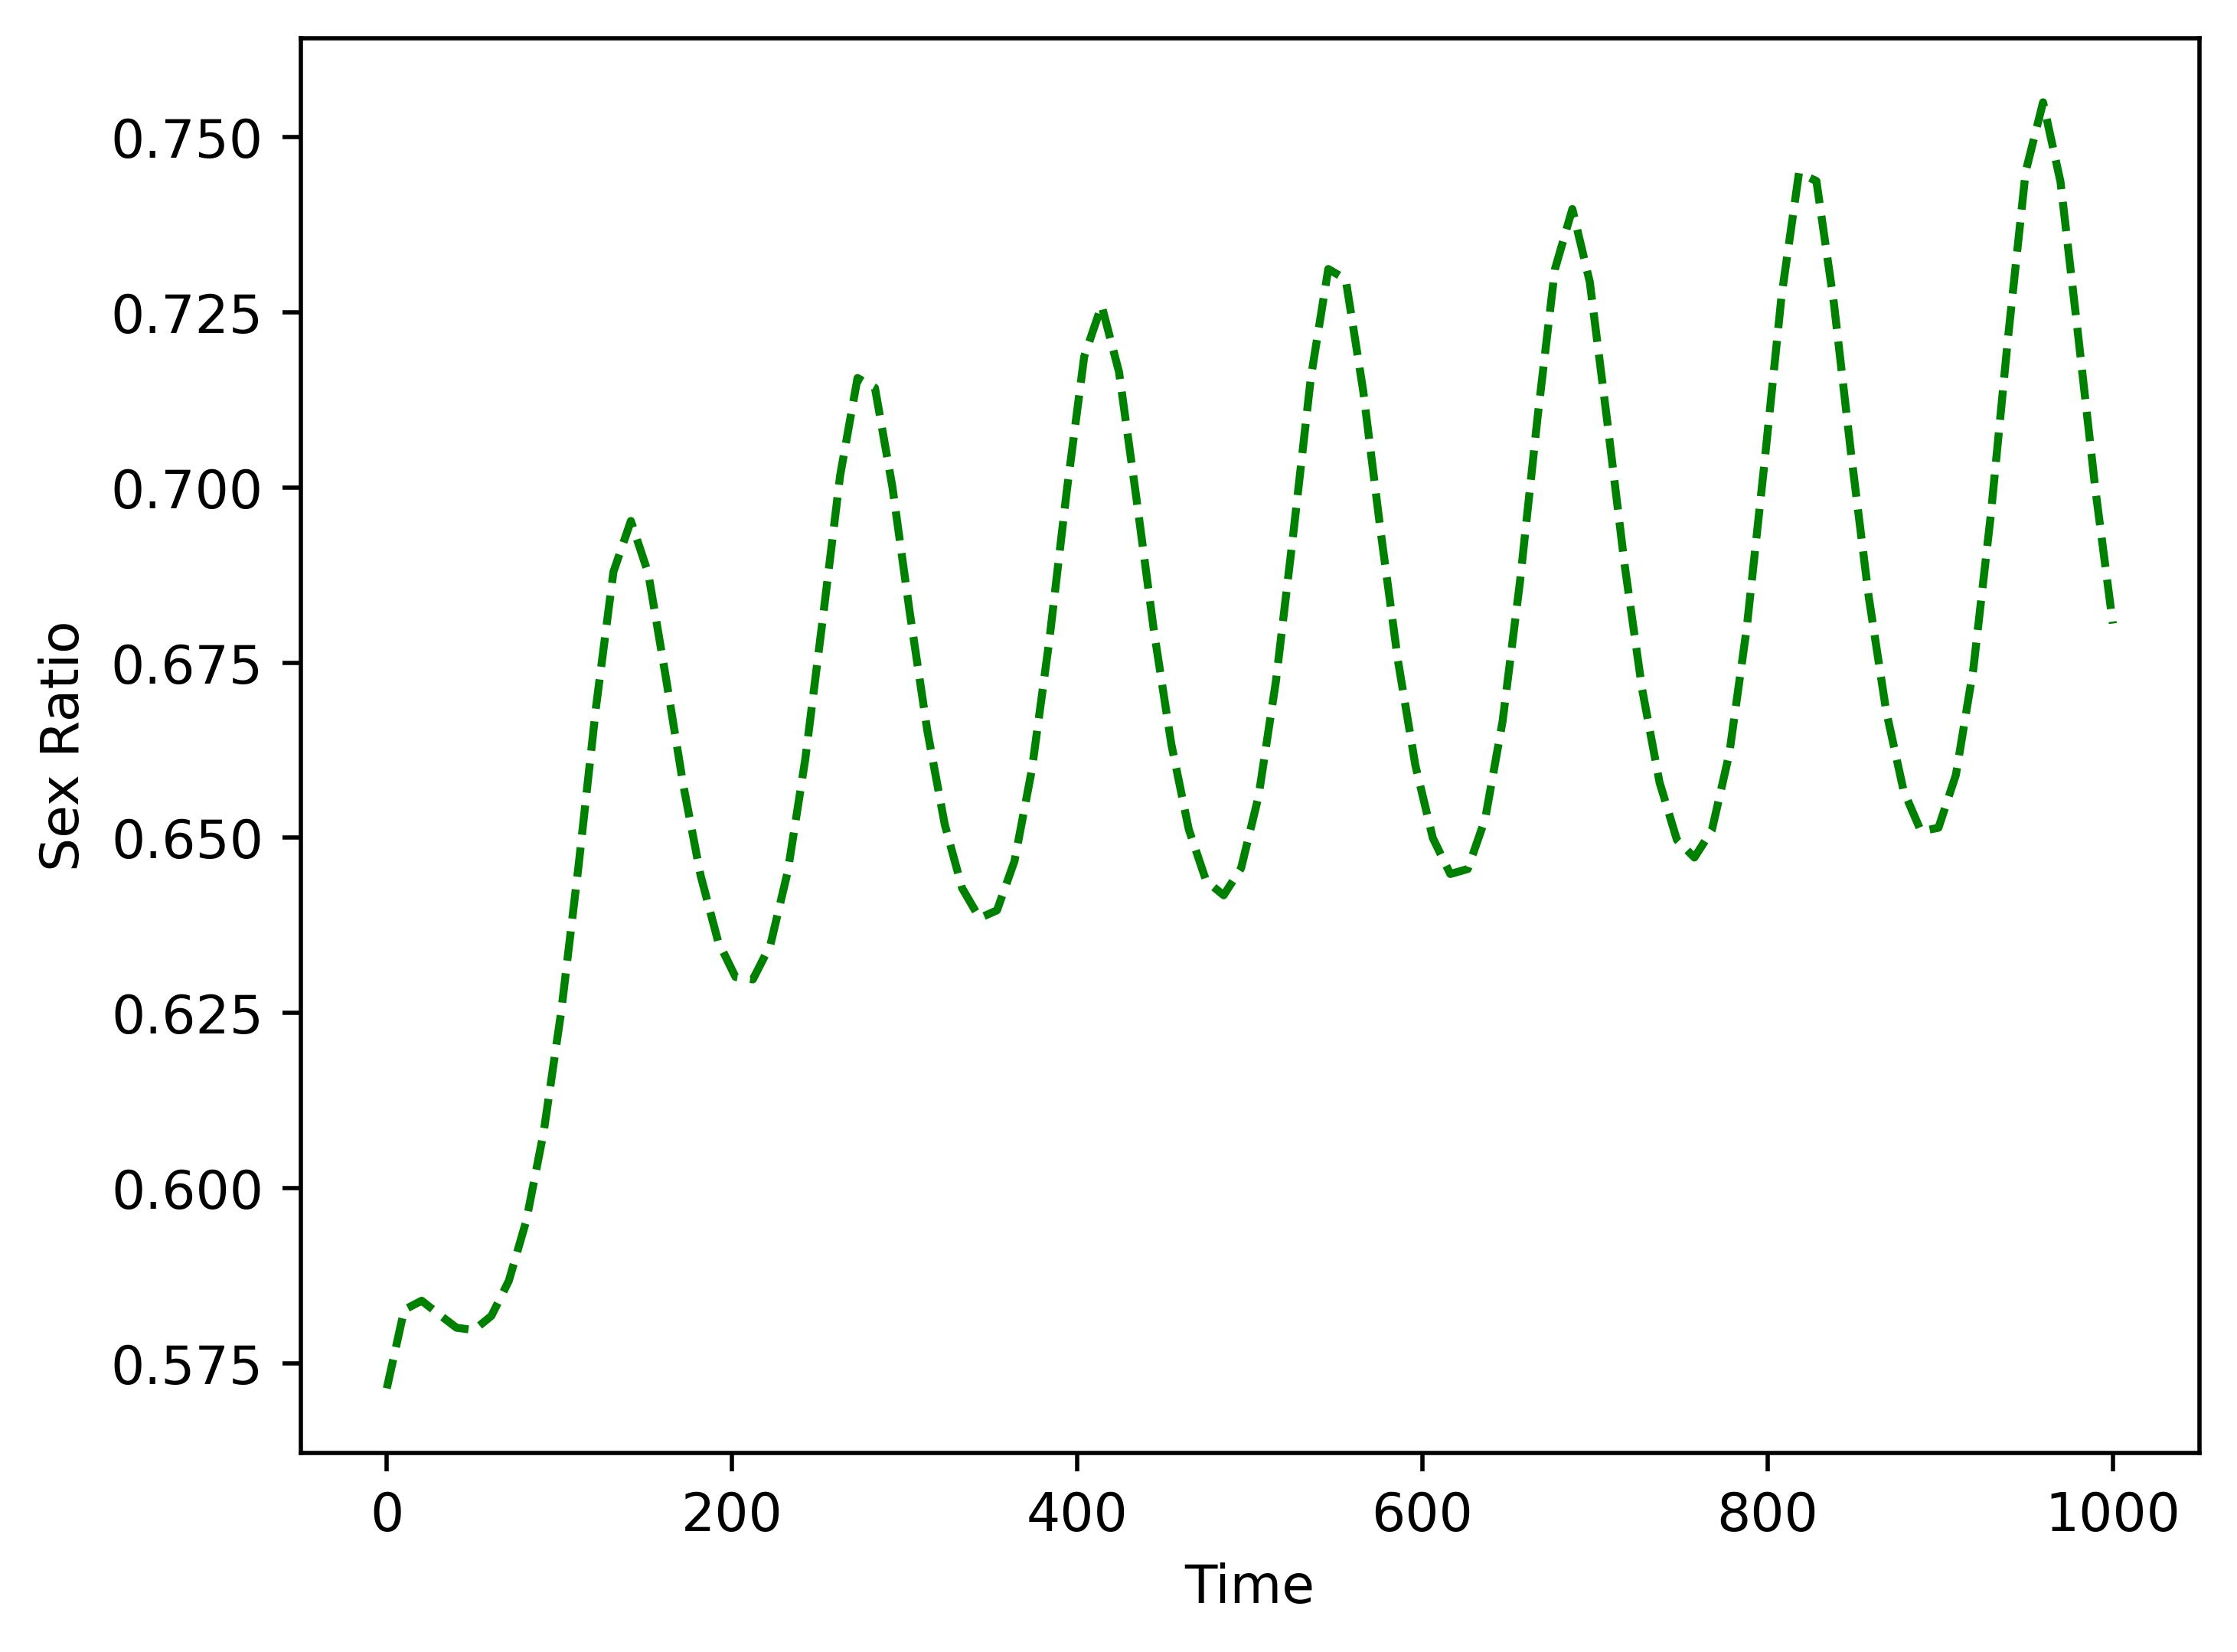
\includegraphics[width=10cm,height=9cm]{Sex_ratio}
     \caption{Sex\_ratio}
     \label{fig:Sex_ratio}
\end{figure}
Simultaneously, we conducted a detailed examination of the gender ratio of seven-gilled sharks over time, and the observed results are illustrated in Figure \ref{fig:Sex_ratio}. From the graph, it is evident that as the prey quantity decreases, the gender ratio of seven-gilled sharks undergoes significant changes. During periods of reduced prey, the proportion of male individuals noticeably increases, reaching approximately 75\%-78\%. This phenomenon suggests that in an environment with scarce prey, male individuals exhibit greater adaptability, and developing into males is advantageous for the continuity of the seven-gilled shark population. Conversely, when prey increases, we observe a decrease in the proportion of male individuals in the gender ratio of seven-gilled sharks, approximately 55\%-60\%. This indicates that under abundant prey resources, female individuals may find it easier to obtain sufficient nutritional support, thereby having better chances of survival and reproduction during the breeding process. Such simulation results are also very consistent with reality, and also reflect that the change in lamprey sex ratio is beneficial to the survival of lampreys.
% 同时,我们进行了对七鳃鳗随着时间变化的性别比例的详细观察,并将观察结果绘制成图\ref{fig:Sex_ratio}。从图中可以明显看出,随着猎物数量的减少,七鳃鳗的性别比例表现出显著的变化。在猎物减少的时候,雄性个体的占比明显增加,达到了约75\%-78\%左右。这一现象暗示着七鳃鳗在面临猎物稀缺的环境中,雄性个体更具适应性,发育成雄性有利于七鳃鳗种族的延续。相反,当猎物增加时,我们观察到七鳃鳗的性别比例中雄性个体的占比降低,约为55\%-60\%左右。这表明,在充足的猎物资源下,雌性个体可能更容易获得足够的营养支持,从而在繁殖过程中具有更好的生存和繁衍机会。这样的模拟结果与实际也非常符合,也体现了七鳃鳗性别比例改变这一特点有利于七鳃鳗的生存。


\begin{figure}[htbp]
       \centering    
   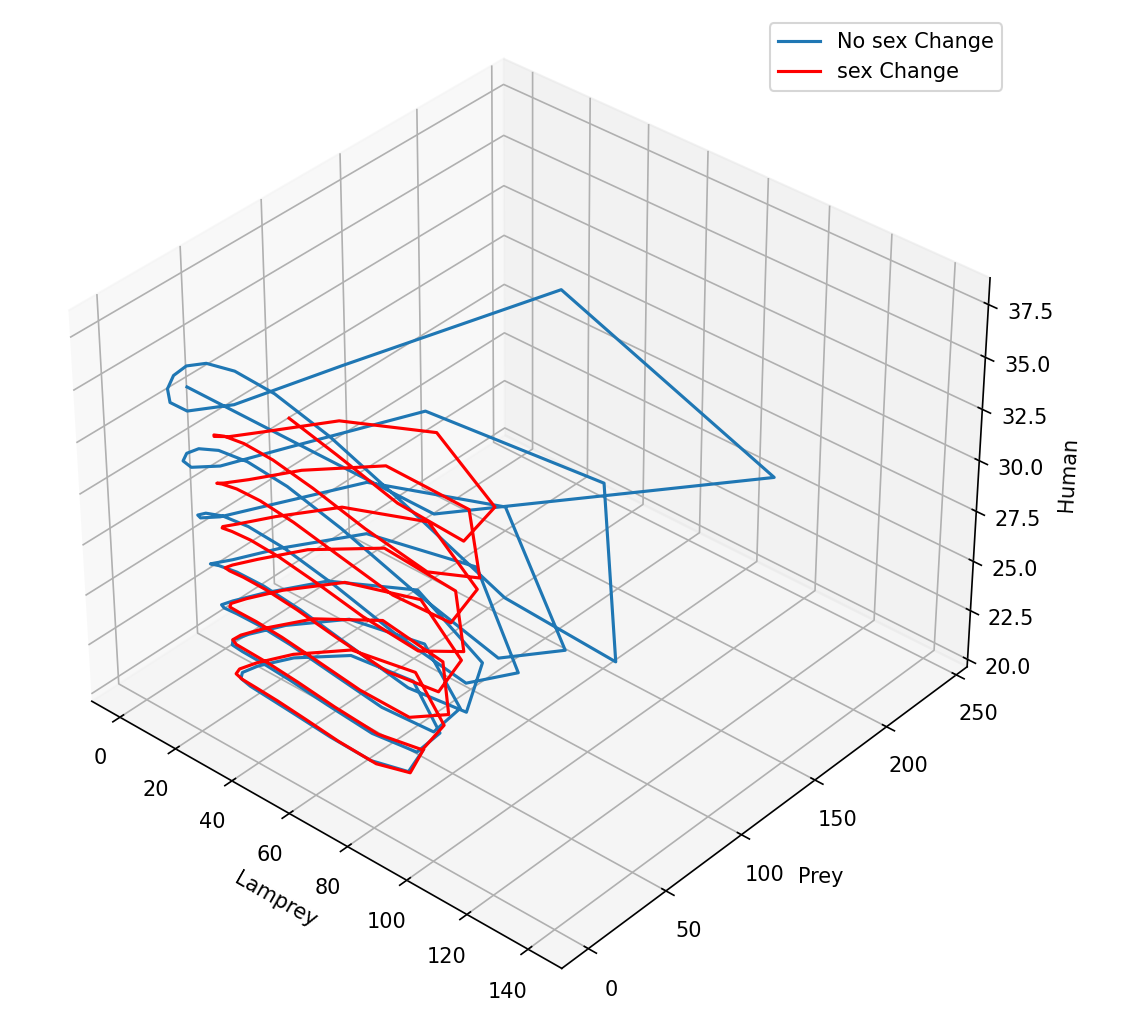
\includegraphics[width=11cm,height=10cm]{Phase_trajectories}
     \caption{Phase\_trajectories}
     \label{fig:Phase_trajectories}
\end{figure}

% 为了深入讨论七鳃鳗性别比例变化与整个食物链的关系,我们进行了两组仿真实验。首先,一组模拟中,我们采用了先前提到的概率公式,将七鳃鳗的发育性别比例$Z_m$设置为随环境变化的概率分布。与此相对比的是第二组仿真实验,我们将七鳃鳗的发育性别比例$Z_m$固定为常数值0.5,代表性别比例不受环境变化的影响。

% 通过绘制相轨图(图\ref{fig:Phase_trajectories}),我们得到了一些引人深思的结果。在性别比例能够变化的情况下,整个食物链系统呈现出高度的稳定性。猎物、七鳃鳗和人类之间的数量交替增减形成了生物圈中的动态平衡。这种相互作用与环境变化相协调,使得生态系统在演化中保持相对稳定。

% 相反,当我们固定七鳃鳗的性别比例不随环境改变时,整个生物链系统逐渐呈现异常趋势。这种缺乏适应性的性别比例可能导致七鳃鳗个体在不同环境下无法有效地调整生存策略,从而影响整个食物链的平衡。这异常趋势可能引发生态系统的不稳定,最终导致生态系统的崩溃。这一仿真实验结果强调了七鳃鳗性别比例对整个食物链系统稳定性的重要性。

To delve deeper into the discussion on the relationship between the changes in the gender ratio of seven-gilled sharks and the entire food chain, we conducted two sets of simulation experiments. In the first set, we employed the probability formula mentioned earlier to set the developmental gender ratio $Z_m$ of seven-gilled sharks as a probability distribution that varies with the environment. In contrast, the second set of simulation experiments involved fixing the developmental gender ratio $Z_m$ of seven-gilled sharks to a constant value of 0.5, representing a gender ratio unaffected by environmental changes.

By plotting phase trajectory diagrams Figure \ref{fig:Phase_trajectories}, we obtained some thought-provoking results. When the gender ratio is allowed to vary, the entire food chain system exhibits high stability. The alternating increase and decrease in the quantities of prey, seven-gilled sharks, and humans form a dynamic equilibrium within the ecosystem. This interaction, coordinated with environmental changes, enables the ecosystem to maintain relative stability during evolution.

On the contrary, when we fixed the gender ratio of seven-gilled sharks without considering environmental changes, the entire food chain system gradually displayed anomalous trends. This lack of adaptive gender ratio may hinder individual seven-gilled sharks from effectively adjusting their survival strategies in different environments, thereby affecting the balance of the entire food chain. This anomaly could trigger instability in the ecosystem, ultimately leading to its collapse. The results of this simulation experiment emphasize the importance of the gender ratio of seven-gilled sharks in maintaining the stability of the entire food chain system.

\subsection{Model 2: Cellular Automaton}
% 模型1我们讨论性别比例对食物链的影响,为了更好理解七鳃鳗对整个生态系统影响,我们使用元胞自动机模拟七鳃鳗对其栖息地的影响。
Model 1 We discuss the impact of sex ratio on the food chain. In order to better understand the impact of lamprey on the entire ecosystem, we use cellular automata to simulate the impact of lamprey on its habitat.
\subsubsection{Description of Cellular Automaton}

Cellular automaton \AIcite{AI2}is essentially an idealized model of a discrete dynamical system, where cells are discrete and finite in both space and time, and their states are also finite. According to the context, the behavior and rules of the cellular automaton model constructed in this paper are as follows:

The cells are located on a two-dimensional grid, representing the entire ecosystem in a 200x200 grid. Each individual cell is considered as one of the possible habitats for the seven-gilled shark. The state of a cell takes into account its four neighbors: front, back, left, and right. The boundary conditions are set as fixed boundary conditions. Each cell randomly generates a value representing the amount of resources in that location. At the beginning, a random location is chosen as the entry point for the seven-gilled shark to enter the ecosystem.
%元胞自动机本质上是一种理想的离散动力学系统模型,其元胞在空间和时间上是离散有限的,元胞的状态也是有限的。根据题意,本文构建的元胞自动机模型行为和规则如下:
%元胞位于二维网格,将整个生态系统作为200x200方格,单个元胞看作七鳃鳗可能的栖息地,元胞的状态考虑前,后,左,右四个邻居,边界条件取固定边界条件,每个元胞随机生成值代表该地的资源量,开始时随机生成一处为七鳃鳗开始进入生态系统的地方。

%该元胞的更新规则:
% (1) 根据当地资源值Res使用计算出七鳃鳗的性别比例$Z_m$,再根据性别比例计算出繁殖率$B$,同时计算出七鳃鳗的数量N。
The update rules for this cellular automaton are as follows:

(1) Calculate the gender ratio $Z_m$ of the seven-gilled shark based on the local resource value Res. Then, calculate the reproduction rate $B$ based on the gender ratio. Simultaneously, determine the population size N of the seven-gilled sharks.
\begin{equation}
\begin{aligned} 
Z_m &= \alpha \cdot {\rm res} + 0.5 \\
B &= Z_m \cdot (1 - Z_m) \cdot c \\
N_{\rm next} &= N + B - \theta * {\rm res}\\
\end{aligned}
\end{equation}

% (2) 根据该地七鳃鳗数量减少该地资源量。
(2) Reduce the resource quantity in a particular location based on the decrease in the population of seven-gilled sharks at that location.

$${\rm Res}_{\rm next} = {\rm Res} - N \cdot \beta + \sigma$$

% (3) 当该地的七鳃鳗数量N大于该地资源所能承受的时候,就会考虑向前,后,左,右进行繁殖,当前,后,左,右资源不为0时,从而增加新元胞。
(3) When the population N of seven-gilled sharks at a specific location exceeds the carrying capacity of the resources at that location, consider reproduction towards the front, back, left, and right directions. Reproduction occurs only in directions where the resources are non-zero, leading to the addition of new cells.

\subsubsection{Result}
\begin{figure}[htbp]
       \centering    
   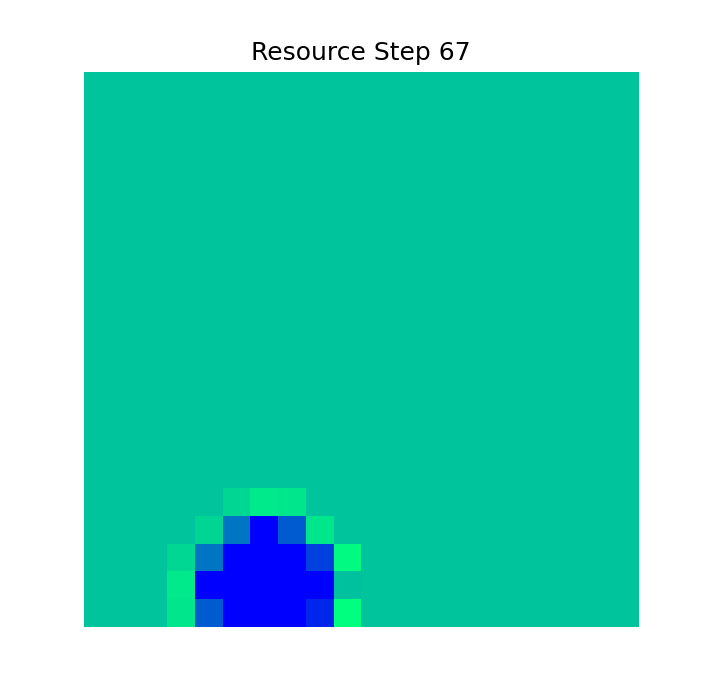
\includegraphics[width=8cm,height=8cm]{Res_step}
     \caption{Cellular automaton simulation diagram}
     \label{fig:Res_step}
\end{figure}

In Figure \ref{fig:Res_step}, the cellular automaton was executed to simulate the relationship between the reproduction of lampreys and their habitat. After 80 iterations, we obtained the simulation results.
% 如图\ref{fig:Res_step},运行元胞自动机模拟七鳃鳗繁殖与栖息地之间关系。通过80次迭代,我们得到模拟结果。
  
% 我们通过两组模拟实验,模拟了丰富和贫瘠资源条件下的情境,并通过元胞自动机得到了相关仿真结果。在资源丰富地区的仿真结果,如图\ref{fig:resource_most}所示,当七鳃鳗的性别比例保持不变时,其种群增长更为迅速,但也伴随着更大的资源消耗。尽管这种性别比例的不变有助于七鳃鳗的繁殖,但其过度的资源消耗可能对整个生态系统造成负面影响。若不予以控制,这种高速增长可能引发生态系统的崩溃。
Through two sets of simulated experiments, we simulated scenarios under conditions of abundant and scarce resources, obtaining relevant simulation results through cellular automata. In the simulation results for resource-abundant areas, as shown in Figure \ref{fig:resource_most}, when the gender ratio of lampreys remains unchanged, their population grows more rapidly, but it is accompanied by greater resource consumption. Although the stability of this gender ratio contributes to the reproduction of lampreys, excessive resource consumption may have negative impacts on the entire ecosystem. If not controlled, this rapid growth could lead to the collapse of the ecosystem.

% 与之相反,在资源贫瘠地区的仿真结果,如图\ref{fig:resource_less}所示,在恶劣的环境条件下,性别比例发生变化的七鳃鳗增长速度更快。这表明在贫瘠环境中,七鳃鳗的这种性别比例调节特性对其繁殖具有显著的优势。值得注意的是,虽然这种情况下的种群增长相对较慢,但其对生态系统的资源消耗较小,有助于生态系统的稳定和其他生物的繁衍。
Contrary to this, in the simulation results for resource-scarce areas, as illustrated in Figure \ref{fig:resource_less}, lampreys experiencing a change in gender ratio exhibit a faster growth rate in harsh environmental conditions. This suggests that the gender ratio adjustment characteristic of lampreys in resource-poor environments provides a significant advantage for their reproduction. It is worth noting that although the population growth in this scenario is relatively slow, the lower resource consumption contributes to the stability of the ecosystem and the reproduction of other organisms.

\begin{figure}[htbp]
      \centering
      \subfigure[Simulation of resource-rich areas] {
          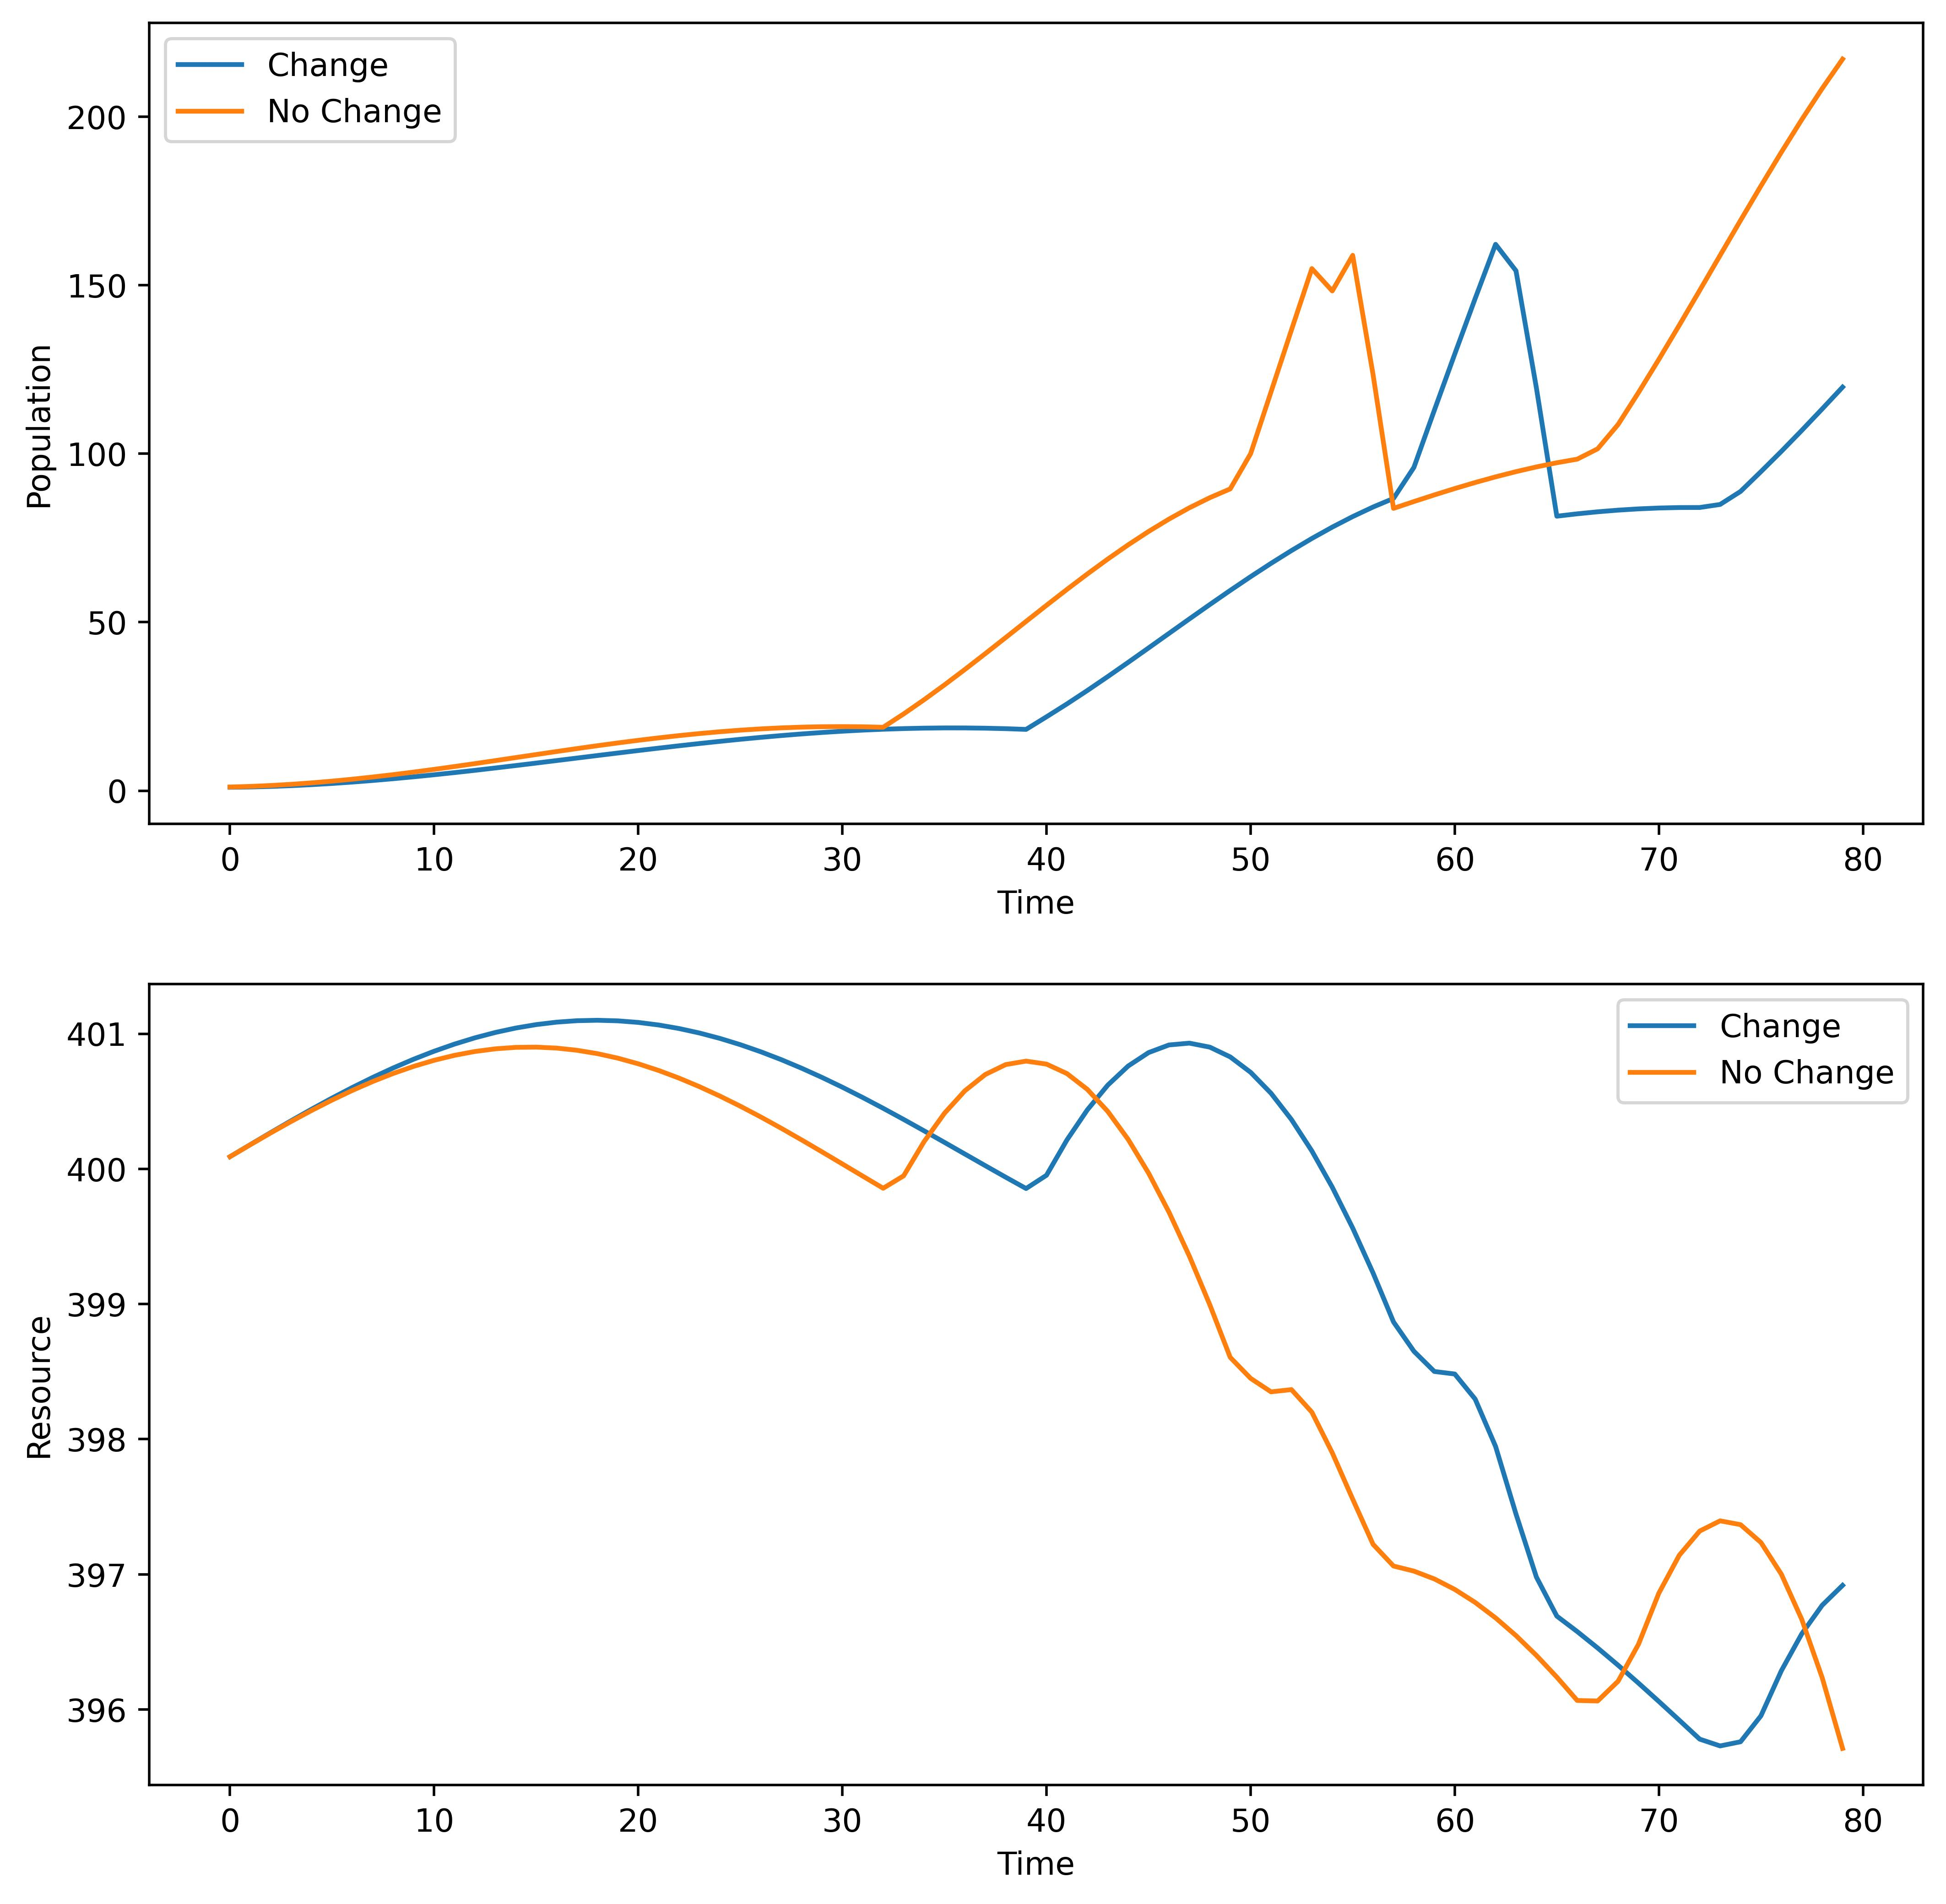
\includegraphics[width=0.4\textwidth]{resource_most}
          \label{fig:resource_most}
      }
       \subfigure[Simulation of resource-poor areas] {
         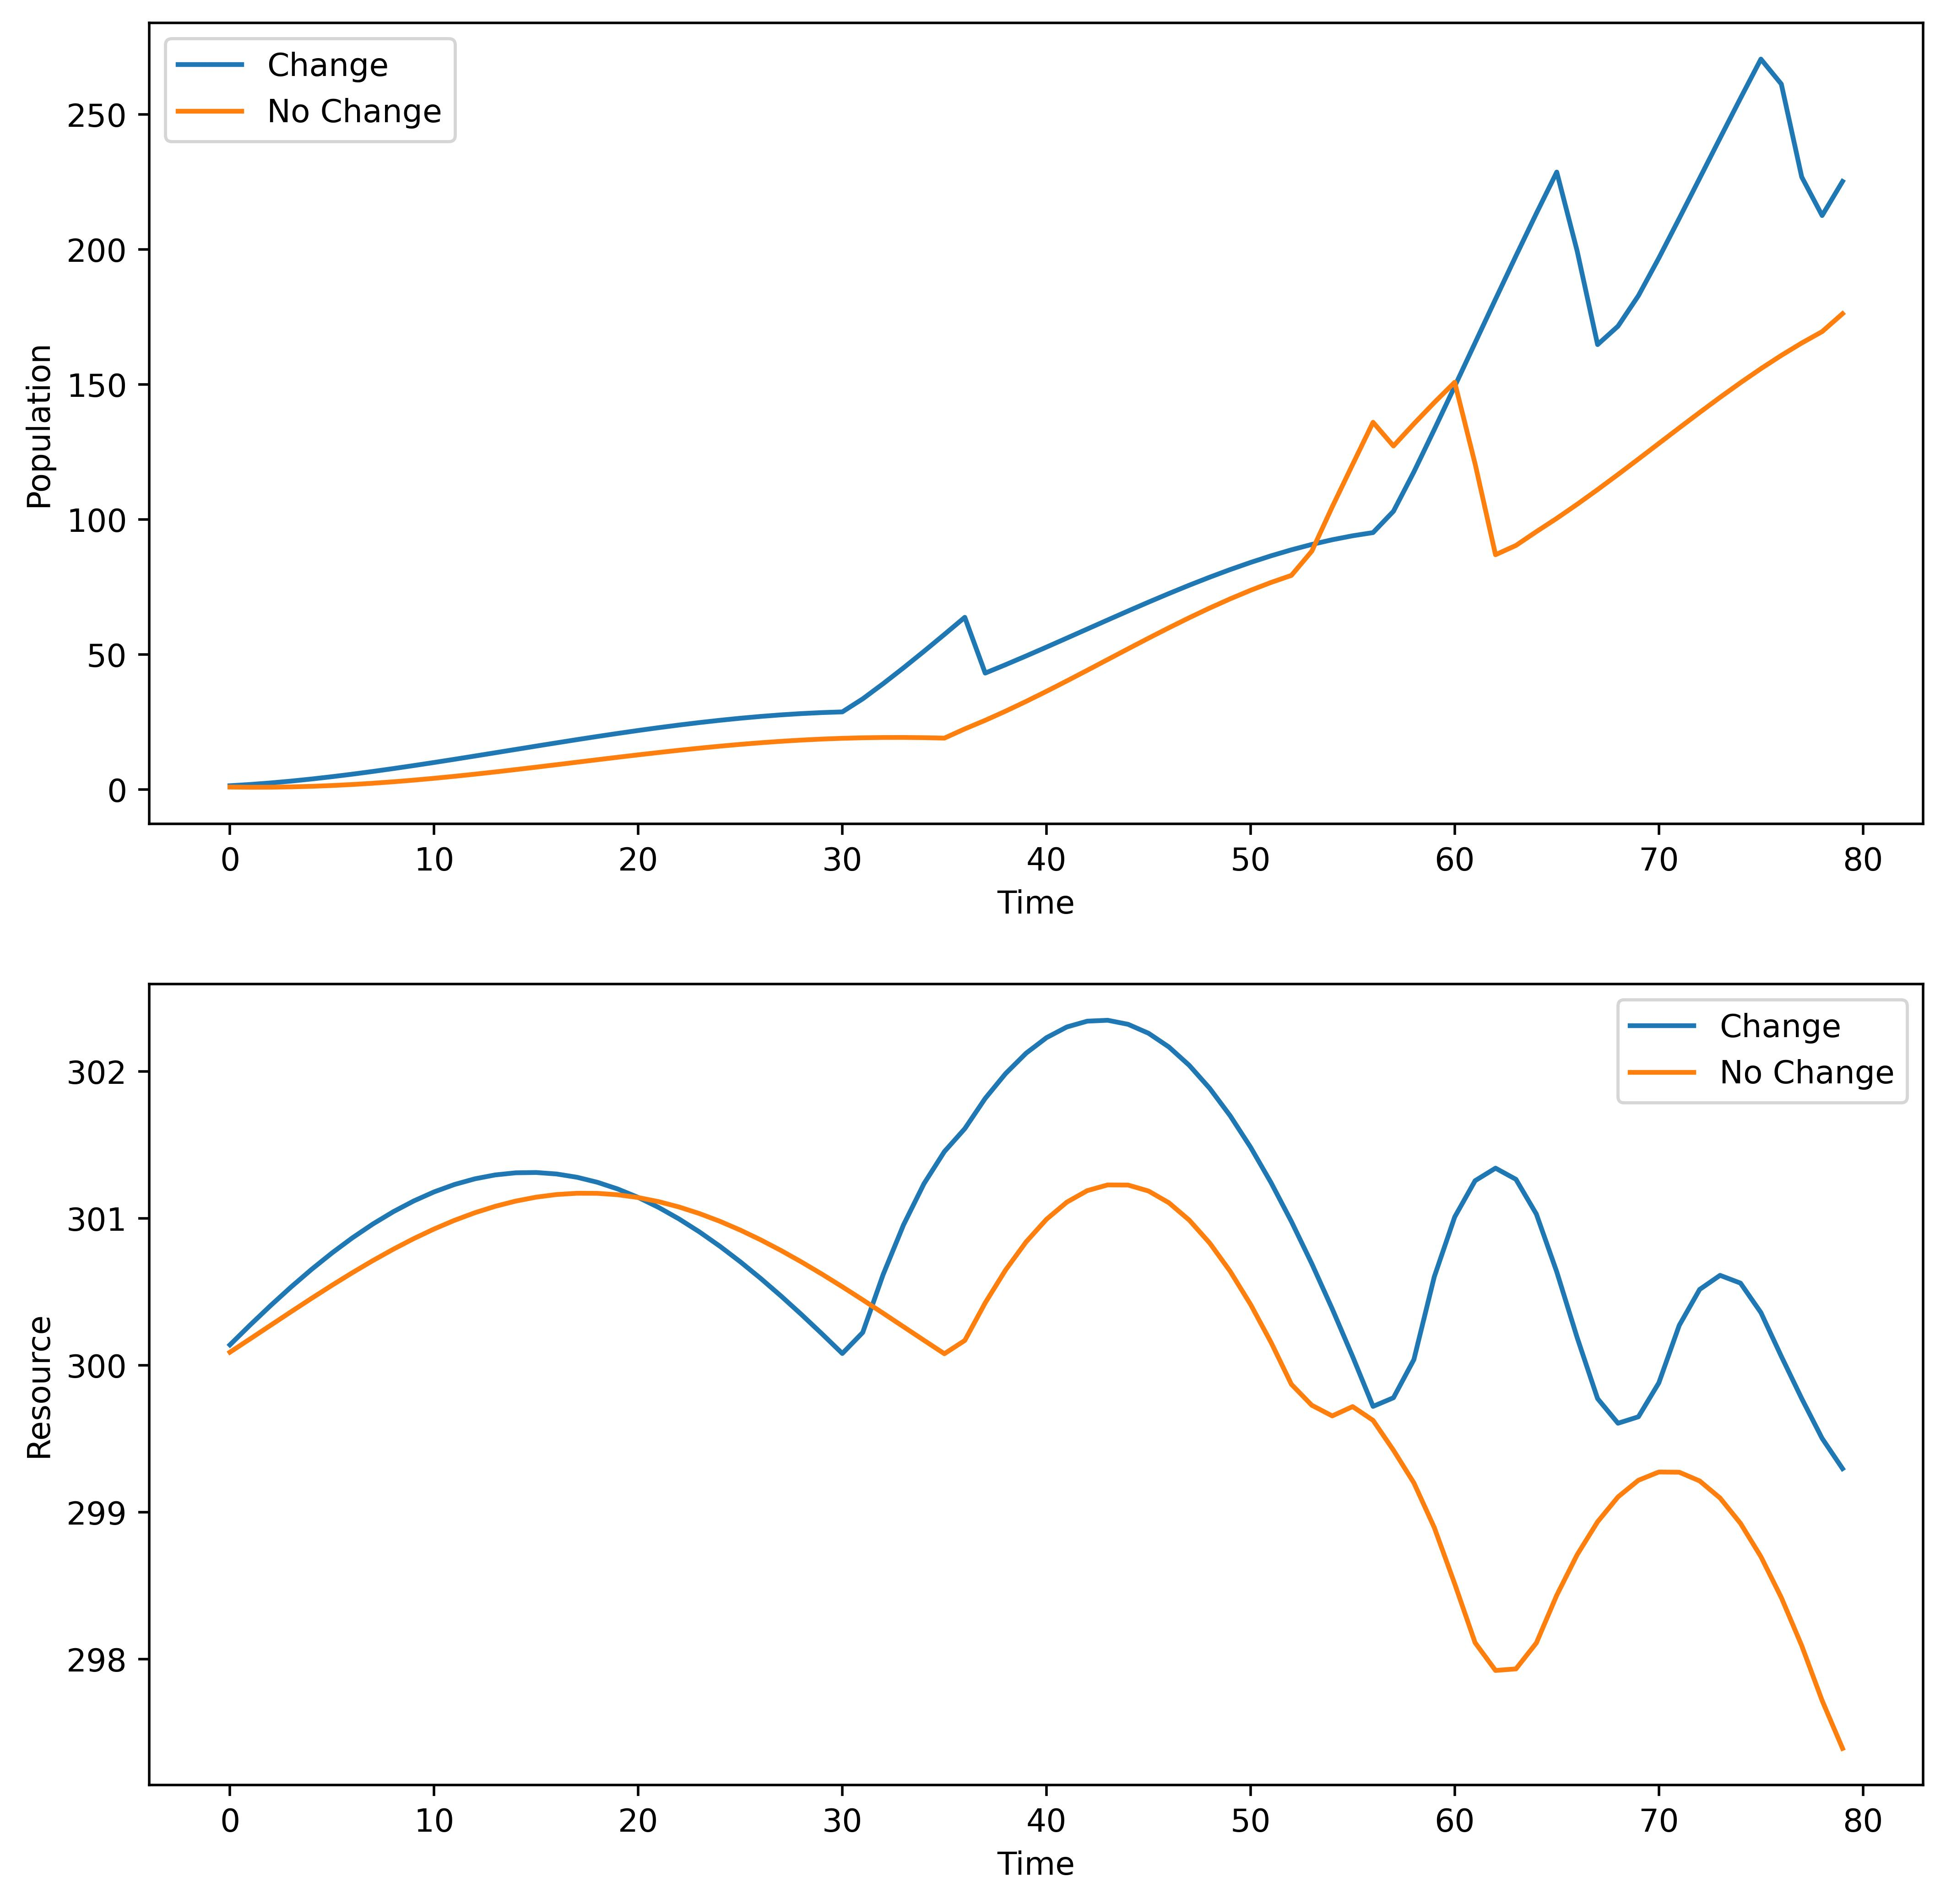
\includegraphics[width=0.4\textwidth]{resource_less}
          \label{fig:resource_less}
      }
\end{figure}
      
  \end{figure}

\subsection{Model 3: Parasitism-host dynamics model}
% \subsection{Model Establishment and Solution for Question four}
We referred to the small parasitic model \cite{Ebert} with vertical transmission established by Ebert et al., combining fundamental infectious disease models and the lamprey population dynamics model established in the first question. We developed a parasitism-host dynamics model specifically for lampreys and obtained the impact curve of gender-altering populations on the parasitic population.
%我们参考了Ebert等人建立的具有垂直传播的小寄生虫模型,结合了基本的传染病模型和第一问建立的七鳃鳗种群动力学模型,建立了针对七鳃鳗的寄生虫-宿主动力学模型,得到了性别改变种群对寄生种群影响曲线。
\subsubsection{Description of Ebert}

The small parasite model developed by Ebert et al. is an epidemiological model using a cross-parasite-species approach that explains the effects of parasites on host population dynamics and allows for an understanding of the variability in host population dynamics in terms of the effects of parasites on host fecundity and survival.Ebert applies to microparasites that are small, unicellular parasites that reproduce directly in the host and are transmitted directly, and all of the microparasites produce persistent infections with no host recovery.
%Ebert等人建立的小寄生虫模型,是使用跨寄生虫物种方法的流行病学模型,能够解释寄生虫对宿主种群动力学影响,能够了解宿主种群动力学中寄生虫对宿主繁殖力和存活影响的可变性。Ebert适用于在宿主内直接繁殖并直接传播的小型单细胞寄生虫的微寄生虫,而且所有微寄生虫都会产生持续感染,而宿主没有恢复。

\begin{equation}
\left\{\begin{aligned} 
  \frac{\mathrm{d} x}{\mathrm{d} t} &=a(x+\theta y)(1-\frac{x+y}{K})-dx-\beta xy   \\  
\frac{\mathrm{d} y}{\mathrm{d} t} &= \beta xy-(d+\alpha ) y
\end{aligned}\right. 
\end{equation}

In this context, \(x(t)\) and \(y(t)\) represent the density of susceptible hosts and infected hosts at time \(t\), respectively. \(a\) is the average growth rate of susceptible hosts, \(\theta\) is the relative reproductive rate of an infected host, \(K\) is the environmental carrying capacity of the host population, \(d\) is the natural death rate of hosts, \(\beta\) is the proportionality coefficient for the infection, and \(\alpha\) is the mortality rate due to parasite-induced effects.
%其中,$x(t)$和$y(t)$分别表示在t时刻易感者和染病宿主的密度;a为易感者宿主的平均增长率;$\theta$为一个染病宿主的相对繁殖率;$K$为宿主种群的环境容纳量;$d$为宿主的自然死亡率;$\beta$为染病的比例系数;$\alpha$为因寄生虫引起的死亡率。

\subsubsection{Our model}
Referring to Ebert's small parasite model and the established model, we developed a parasitism-host dynamics model specifically for lampreys.

%参考EBert的小寄生虫模型和已经建立的模型,我们建立了针对七鳃鳗的寄生虫-宿主动力学模型。
To simulate changes in the gender ratio of lampreys with varying resource levels, we utilized the previously established model and made necessary simplifications.
%为了模拟七鳃鳗性别比例随着资源多少发生变化,在此利用前面建立的模型,并适当做出了必要的简化。

\begin{enumerate}
	 \item Ignored the impact of human predation on lampreys. 
     \item Neglected the influence of interspecies competition on the organisms. 
     \item Assumed consistent infection probabilities and mortality rates for both male and female species. 
     \item Considered that being infected with parasites does not affect the reproductive rate, and reproduction does not transmit parasites to the next generation.
\end{enumerate}
%1.忽略人类的捕食对七鳃鳗的影响。2.忽略物种间的竞争对生物的影响。3.雌雄物种感染寄生虫的概率一致,感染寄生虫的雌雄死亡率一致。4.感染寄生虫并不影响繁殖率,繁殖不会将寄生虫传染给下一代。

Combining these assumptions, we established the following model:
%结合以上的假设我们建立了以下的模型:

\begin{equation}
\begin{aligned}
I &= M_I+F_I   \\
\frac{\mathrm{d} M_R}{\mathrm{d} t} &= BNZ-d_MM_R-kIM_R+b_{11}aPM_R
\end{aligned}
\end{equation}

$N$ is the total population size, $I$ is the total number of infected individuals, $B$ is the birth rate, $Z$ is the probability that a hatchling converts to a male, $M_R$ is the number of susceptible males, $M_I$ is the number of infected males, $F_I$ is the number of infected females, $d_M$ is the natural mortality rate of males, $k$ is the rate of infection, $k_MIM_R$ is the increase in infected individuals, $a$ is the probability that prey $P$ is predated, $b_{11}$ is the predation efficiency of susceptible males, $P$ is the number of predators, and the last term $b_{11}aPM_R$ is the increase in males due to predation.
%$N$是种群的总数量,$I$是总感染者数量,$B$是出生率,$Z$是幼体转化为雄性的概率,$M_R$是雄性易感者的数量,$M_I$是雄性感染者的数量,$F_I$是雌性感染者的数量,$d_M$是雄性自然死亡率,$k$是感染率,$k_MIM_R$是增加的感染者,$a$是猎物$P$被捕食的概率,$b_{11}$是易感染雄性的捕食效率,$P$是被捕食者的数量,最后一项$b_{11}aPM_R$是捕食带来的雄性增长。

\begin{equation}
\begin{aligned}
\frac{\mathrm{d} M_I}{\mathrm{d} t} &= kIM_R-(d_M+d_I)M_I+b_{12}aPM_I 
\end{aligned}
\end{equation}

$M_I$ is the number of infected male,$d_I$ is the infection mortality rate and $b_{12}$ is the predation efficiency of infected males.
%$M_I$是雄性感染者的数量,$d_I$是感染死亡率,$b_{12}$是雄性感染者的捕食效率。

Similarly we can obtain a model of the transmission dynamics of female susceptible and infected individuals:
%同理我们可以得到雌性易感者和感染者的传染动力学模型:

\begin{equation}
\begin{aligned}
\frac{\mathrm{d} F_R}{\mathrm{d} t} &= BN(1-Z)-d_FF_R-kIF_R+b_{21}aPF_R   \\
\frac{\mathrm{d} F_I}{\mathrm{d} t} &= kIF_R-(d_F+d_I)F_I+b_{22}aPF_I 
\end{aligned}
\end{equation}

$d_F$ is the natural mortality rate of females, $F_R,F_I$ is the number of susceptible and infected females, respectively, $d_F$ is the natural mortality rate of females and $b_{21},b_{22}$ is the efficiency of predation by susceptible and infected females.
%$d_F$是雌性的自然死亡率,$F_R,F_I$分别是雌性易感者和感染者的数量,$d_F$是雌性自然死亡率,$b_{21},$b_{22}$$是雌性易感者和感染者捕食效率.

\begin{equation}
\begin{aligned}
N &= M_R+M_I+F_R+F_I   \\
B &= cb(1-b)   \\
b &= \frac{M_R+M_I}{M_R+M_I+F_R+F_I}   \\
Z_{M} &= \frac{\gamma }{1+p^{\alpha } } +\beta 
\end{aligned}
\end{equation}

$c$ is a constant that regulates the birth rate, $Z_M$ is the probability that a hatchling converts to a male, and $\gamma,\alpha,\beta$ are all regulatory constants.
%$c$是调节出生率的常数,$Z_M$是幼体转化为雄性的概率,$\gamma,\alpha,\beta$都是调节常数

The following prey model was used to mimic the seven-gill eel's access to food in nature:
%下面是猎物模型,用来模仿七鳃鳗在自然界获取食物的状况
\begin{equation}
\begin{aligned}
\frac{\mathrm{d} P}{\mathrm{d} t} &= r_pP-aNP-d_pP
\end{aligned}
\end{equation}

where $r_p$ is the natural birth rate of prey and $d_p$ is the natural death rate of prey.
%其中$r_p$是被捕食者的自然出生率,$d_p$是被捕食者的自然死亡率

\subsubsection{Result}

For the aforementioned system of differential equations, we employed the fourth-order Runge-Kutta algorithm for solving.The specific parameters of the model are shown in the following table\ref{Parameter Settings2}.The computed graph is presented in Figure \ref{four}. As the number of parasitic infections in lampreys increases, due to the relatively minor impact of parasites on male lampreys, the population of lampreys adapts by increasing the male ratio to counter the threat of parasites. The gradual increase in the proportion of male lampreys leads to a higher likelihood of parasites choosing to infest male individuals, thereby avoiding the potentially severe consequences of infesting female individuals, such as female mortality.

This unique adaptive behavior allows the lamprey population to survive under the pressure of parasitic threats and maintain a relatively balanced ecosystem. The outcomes of this natural selection contribute to ensuring the coexistence of lamprey populations and parasites, mitigating the threat of extinction.
%对于上述的微分方程组我们采用四阶龙格库塔算法求解,模型具体参数见如下\ref{Parameter Settings2},最终计算出的图如\ref{four}, 随着感染寄生虫的七鳃鳗数量的增加, 由于寄生虫对雄性七鳃鳗的影响较小,七鳃鳗群体提高雄性比例对抗寄生虫的威胁。雄性七鳃鳗的比例逐渐增加,这导致寄生虫更有可能选择寄生到雄性个体身上,而避免了寄生到雌性个体可能导致的严重后果,如雌性的死亡。这一独特的行为适应使得七鳃鳗群体能够在寄生虫压力下存活,并维持相对平衡的生态系统。这种自然选择的结果有助于确保七鳃鳗群体与寄生虫之间的共存,避免了灭亡的威胁。

\begin{table}[htbp]
  \centering
  \label{Parameter Settings2}
  \caption{Parameter Settings2}
  \begin{tabular}{cccc}
   \toprule
    Parameter name & Parameter value & Parameter name & Parameter value\\
    \midrule
    $c$ & 0.08 & $d_I$ & 0.001\\
    \alpha & 0.01 & $d_p$ & 0.1 \\
    \beta & 0.53 & $b_{11}$ & 0.4 \\
    \gamma & 0.3 &  $b_{12}$ & 0.05 \\
    $r_p$ & 0.588 & $b_{21}$ & 0.09 \\
    $d_F$ & 0.04 & $b_{22}$ & 0.04 \\
    $d_M$ & 0.03 & $k$ & 0.001\\   
  \bottomrule
\end{tabular}
\end{table}

\begin{figure}[htbp]
       \centering    
   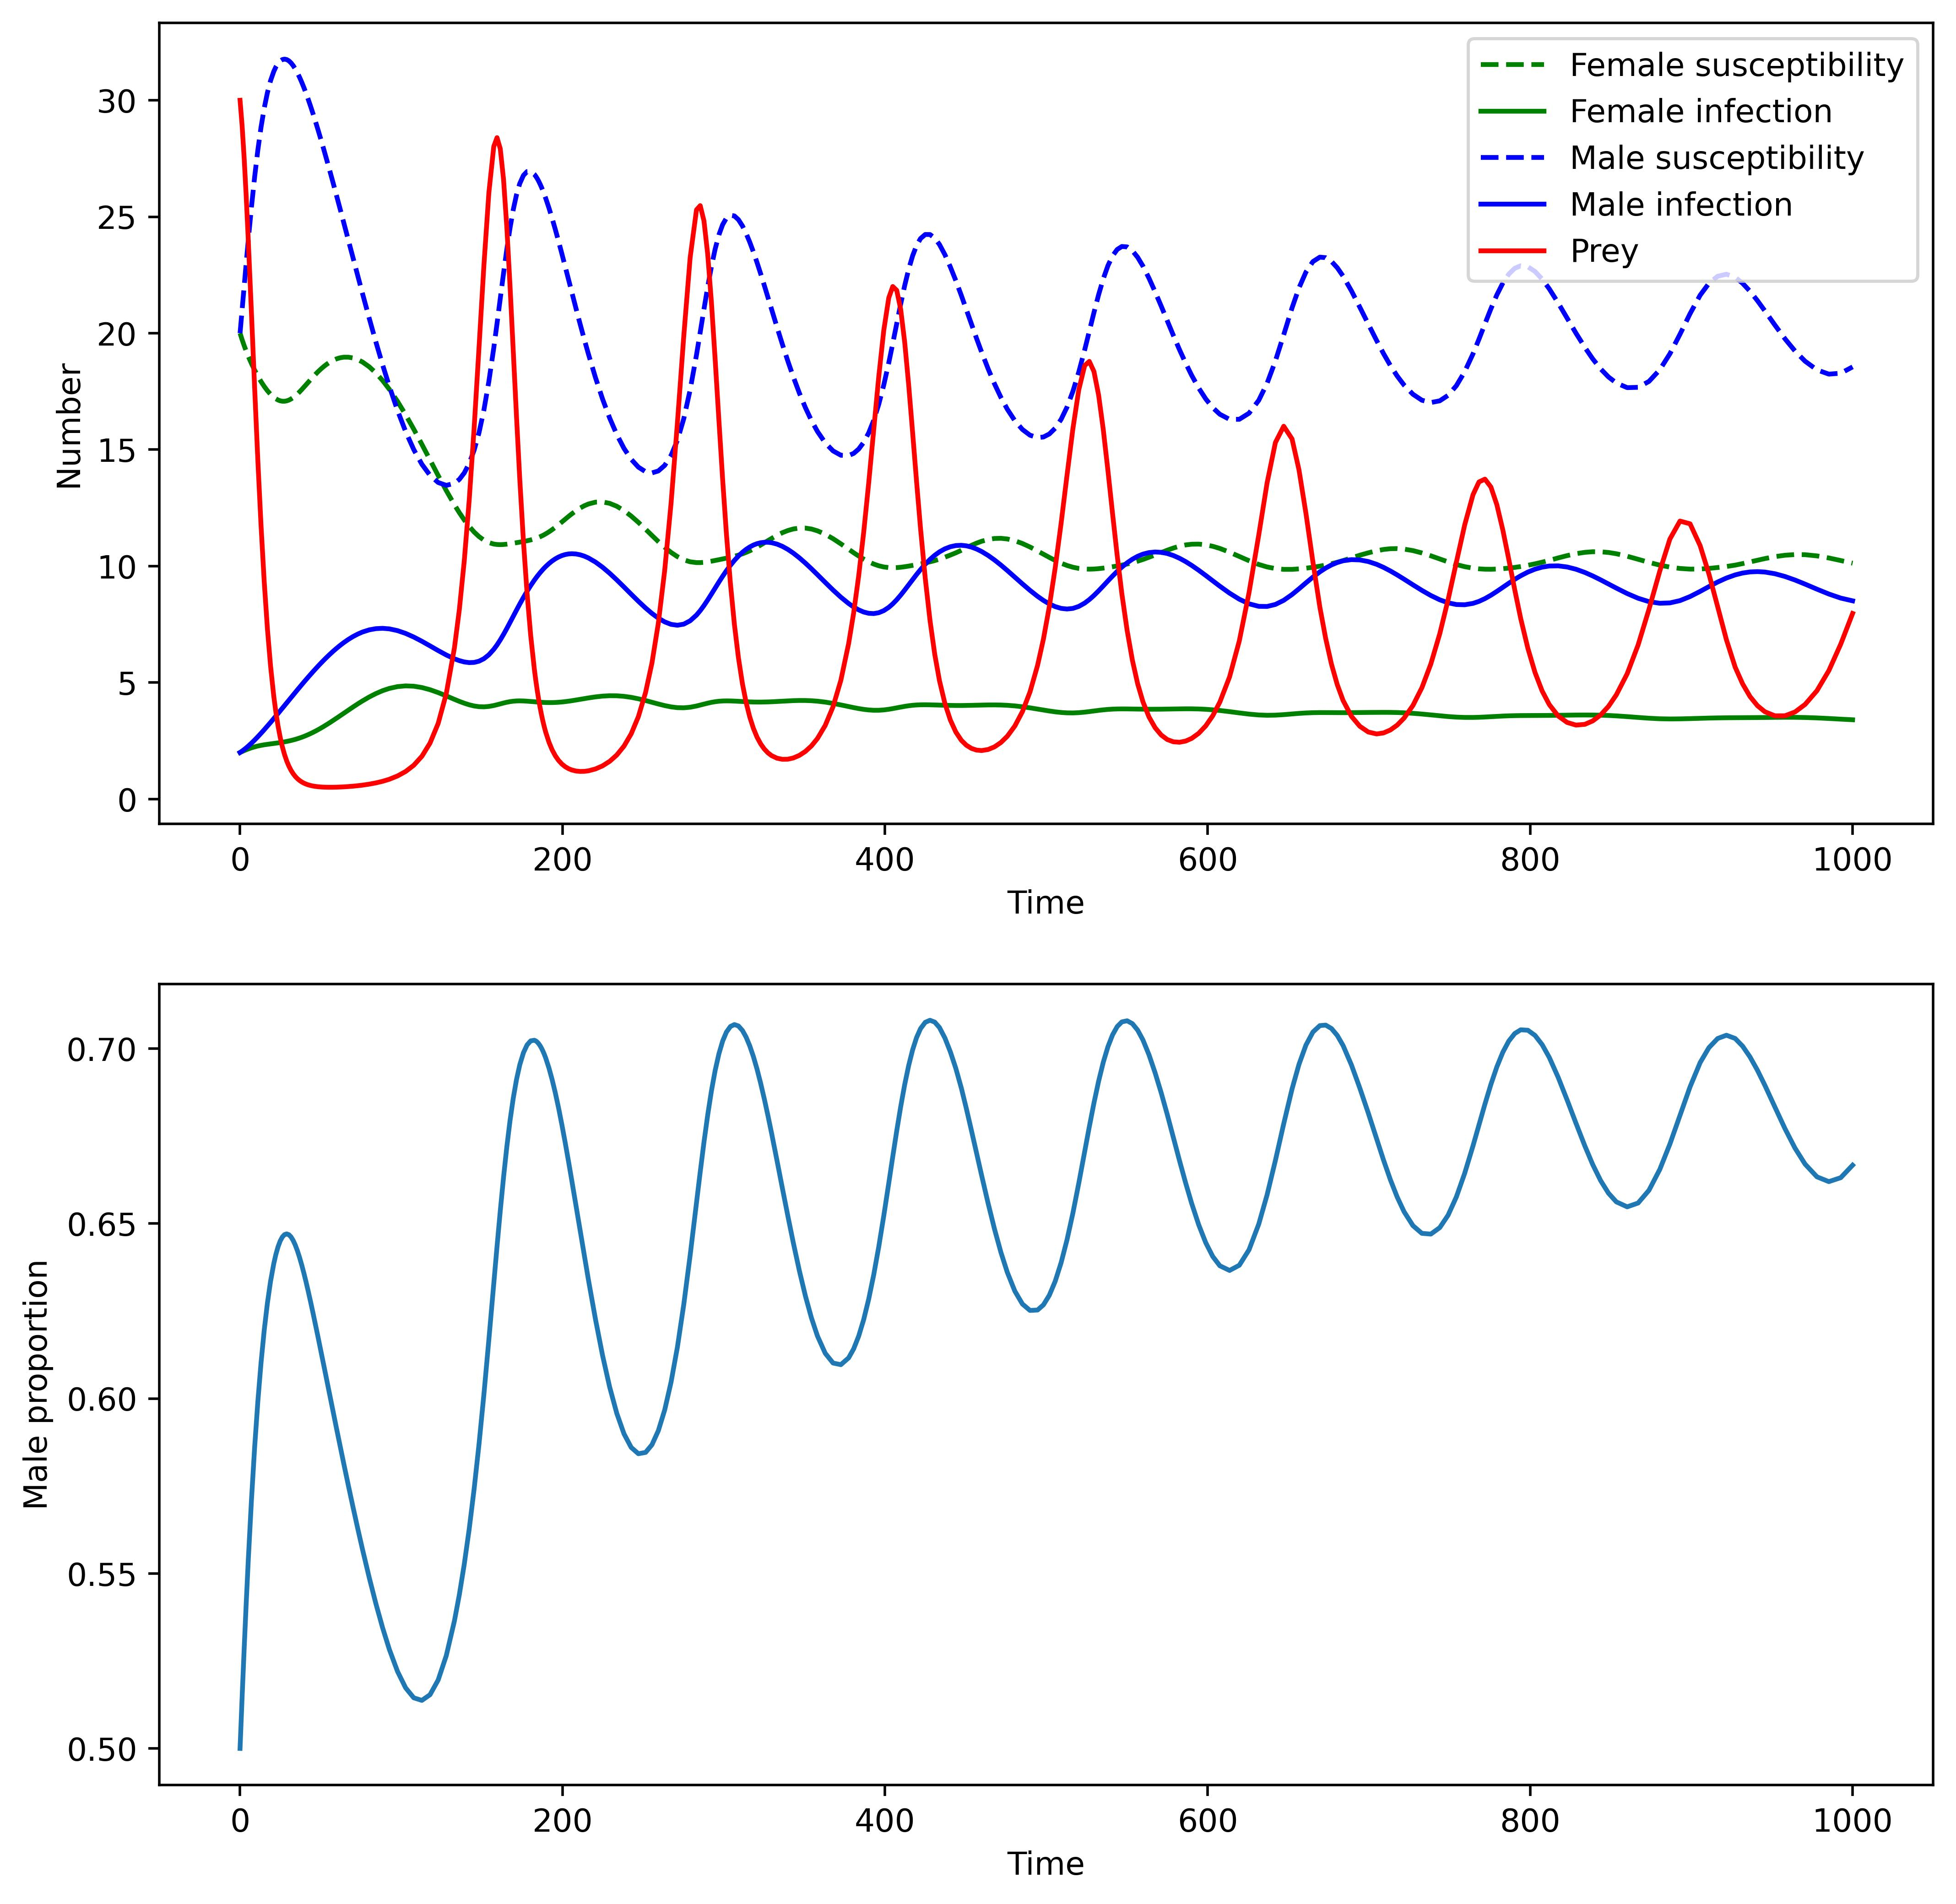
\includegraphics[width=11cm,height=10cm]{four}
     \caption{Parasite-host dynamics calculation results diagram}
     \label{four}
\end{figure}

\section{Sensitivity Analysis}

%在模型1中,我们认为七鳃鳗的种群数量变化是只与自然生存,自然死亡,捕食猎物,被人类捕食四个因素影响,实际上七鳃鳗可能受更多因素影响,所以我们在后面加入扰动项\epsilon, 观察\epsilon的灵敏度.另外控制性转率的\alpha是控制七鳃鳗性别比例的关键参数,所以我们也对其进行灵敏度分析.对于灵敏度分析,我们设定七鳃鳗种群在食物链的最多存活时间$T_{max}$后,种群数$N$为0,并以此为指标.
In Model 1, we assumed that the population dynamics of lampreys are influenced only by four factors: natural birth, natural death, predation, and human harvesting. In reality, lampreys may be affected by more factors. Therefore, we introduced a perturbation term \(\epsilon\) in subsequent models to observe the sensitivity to \(\epsilon\). Additionally, the control parameter \(\alpha\), governing the sex ratio of lampreys, is a critical factor. Hence, we conducted sensitivity analysis on \(\alpha\).

For sensitivity analysis, we set the lamprey population to reach zero after a maximum survival time \(T_{max}\) in the food chain, using this as an indicator.

\begin{figure}[htbp]
      \centering
      \subfigure[$\epsilon$ sensitivity analysis] {
          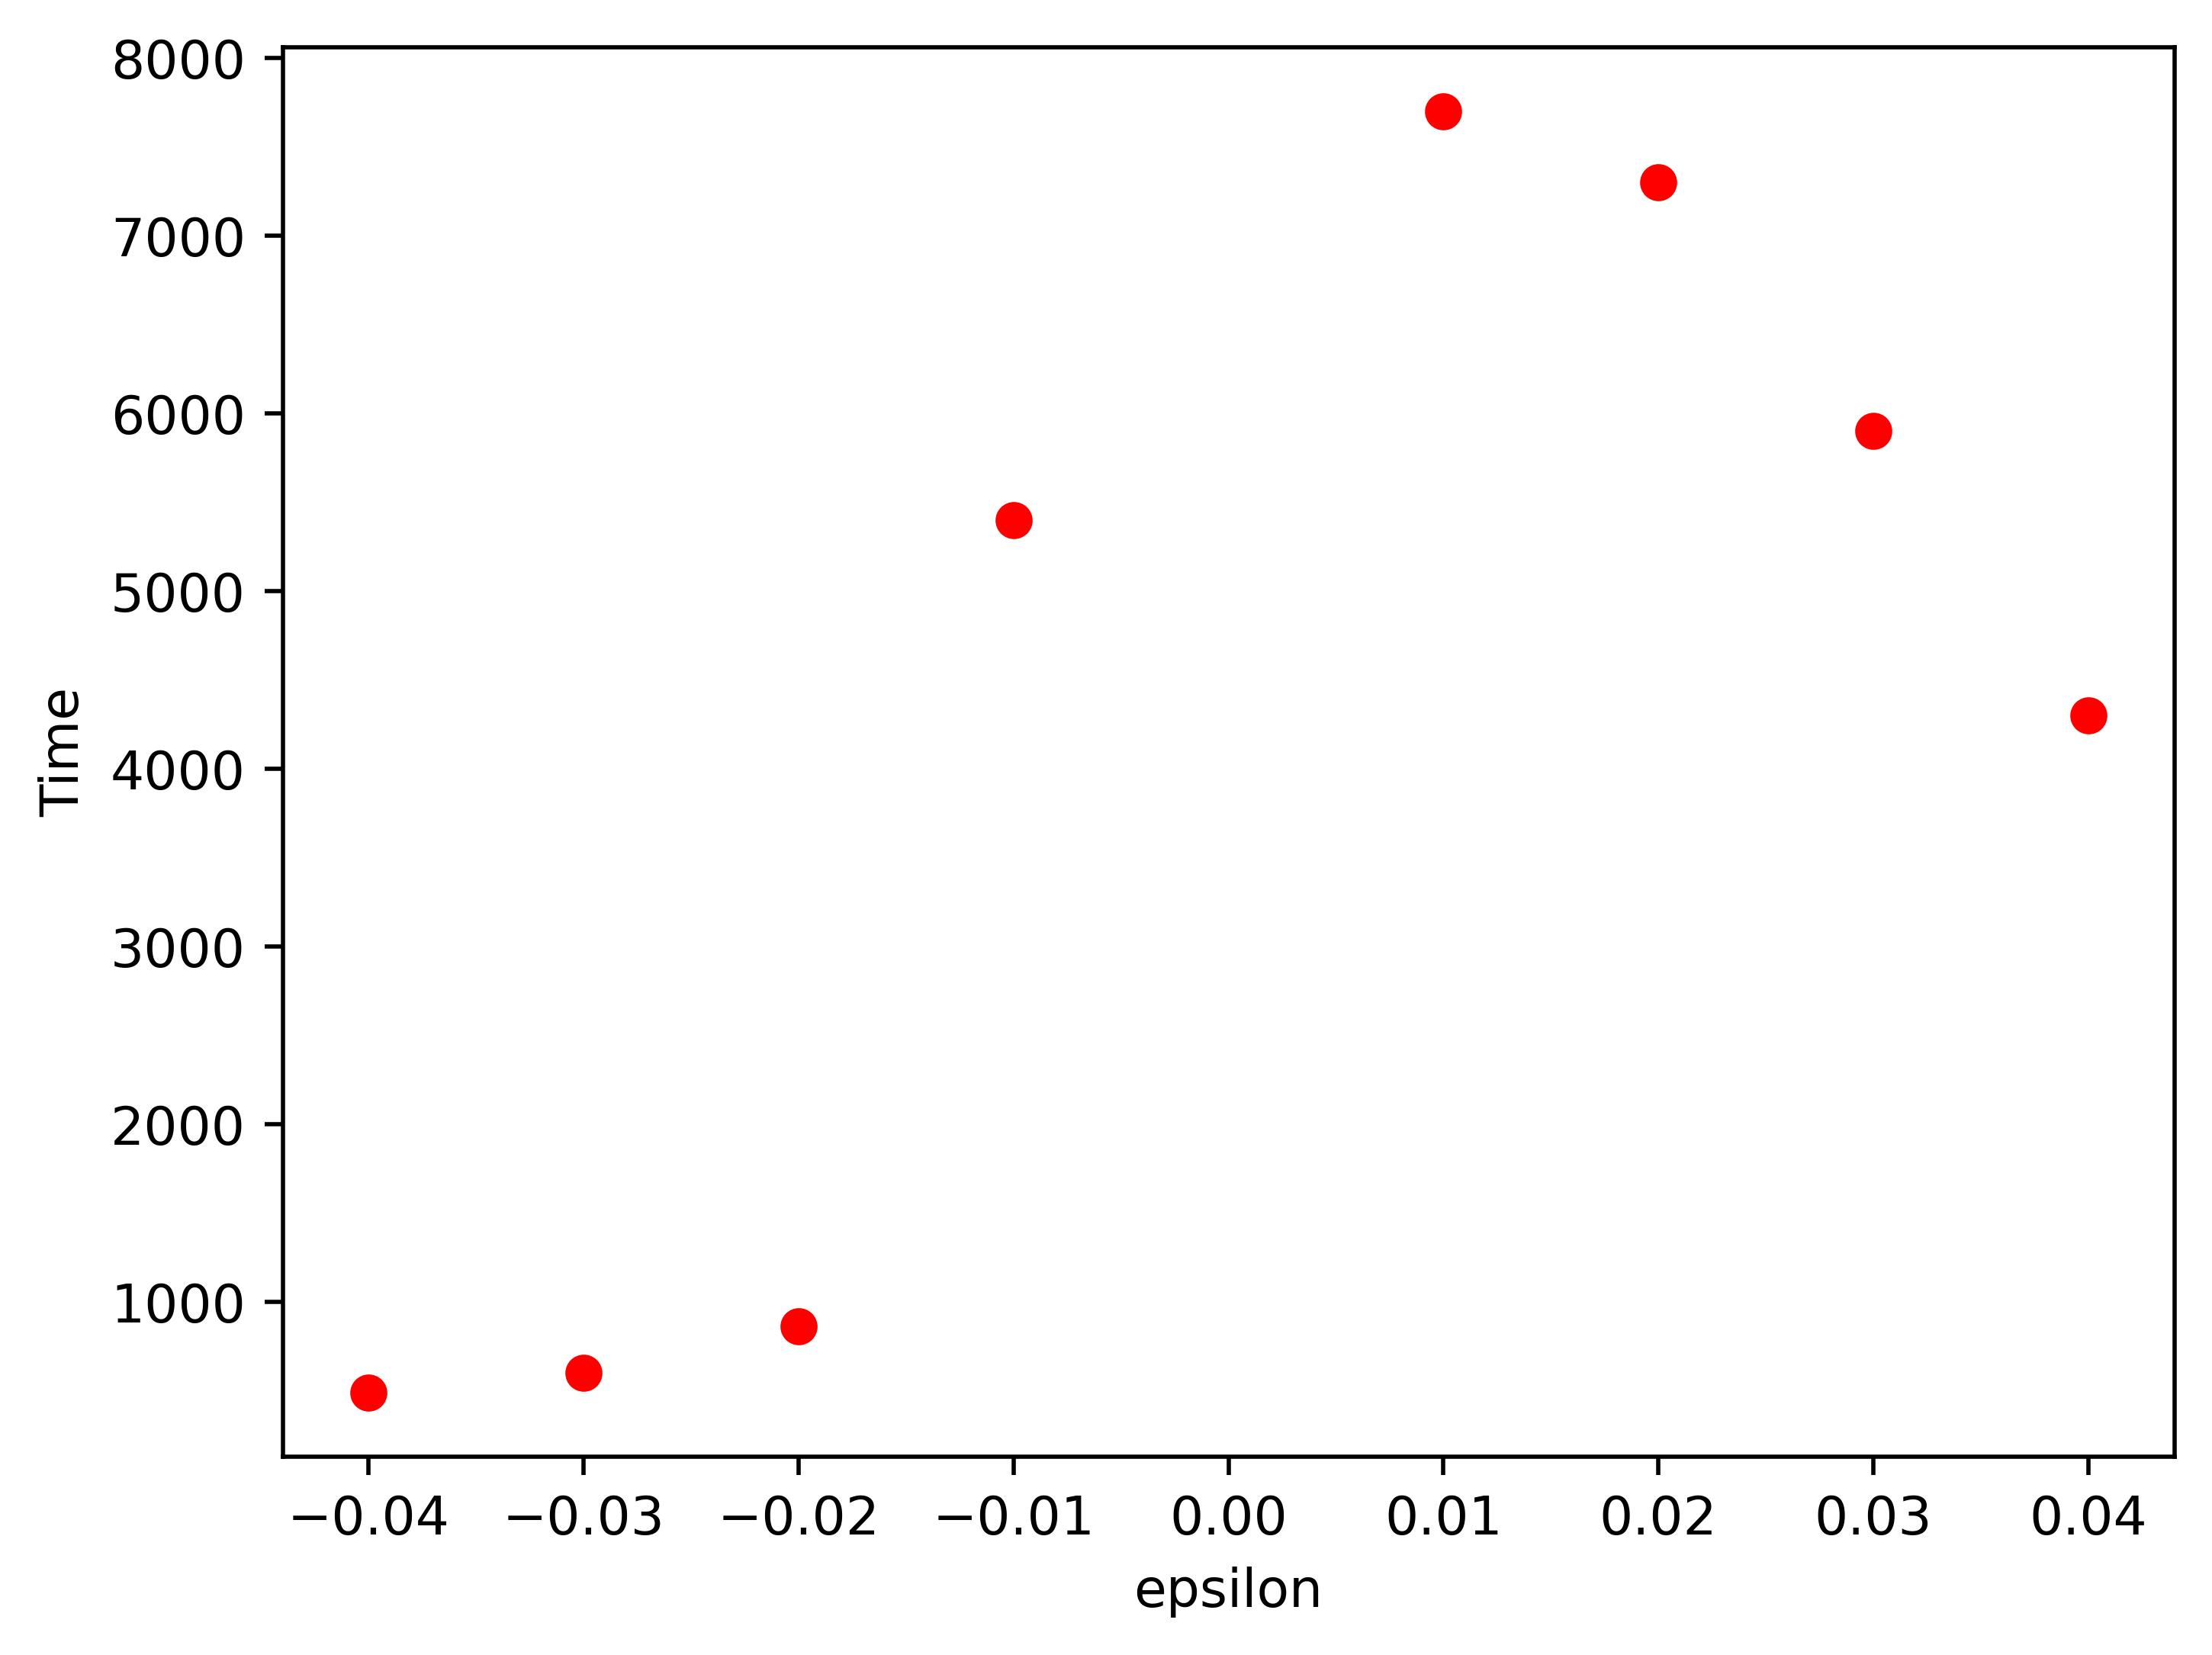
\includegraphics[width=0.4\textwidth]{SA1}
          \label{fig:Sensitivity_Analysis_1}
      }
      \subfigure[$\alpha$ sensitivity analysis] {
         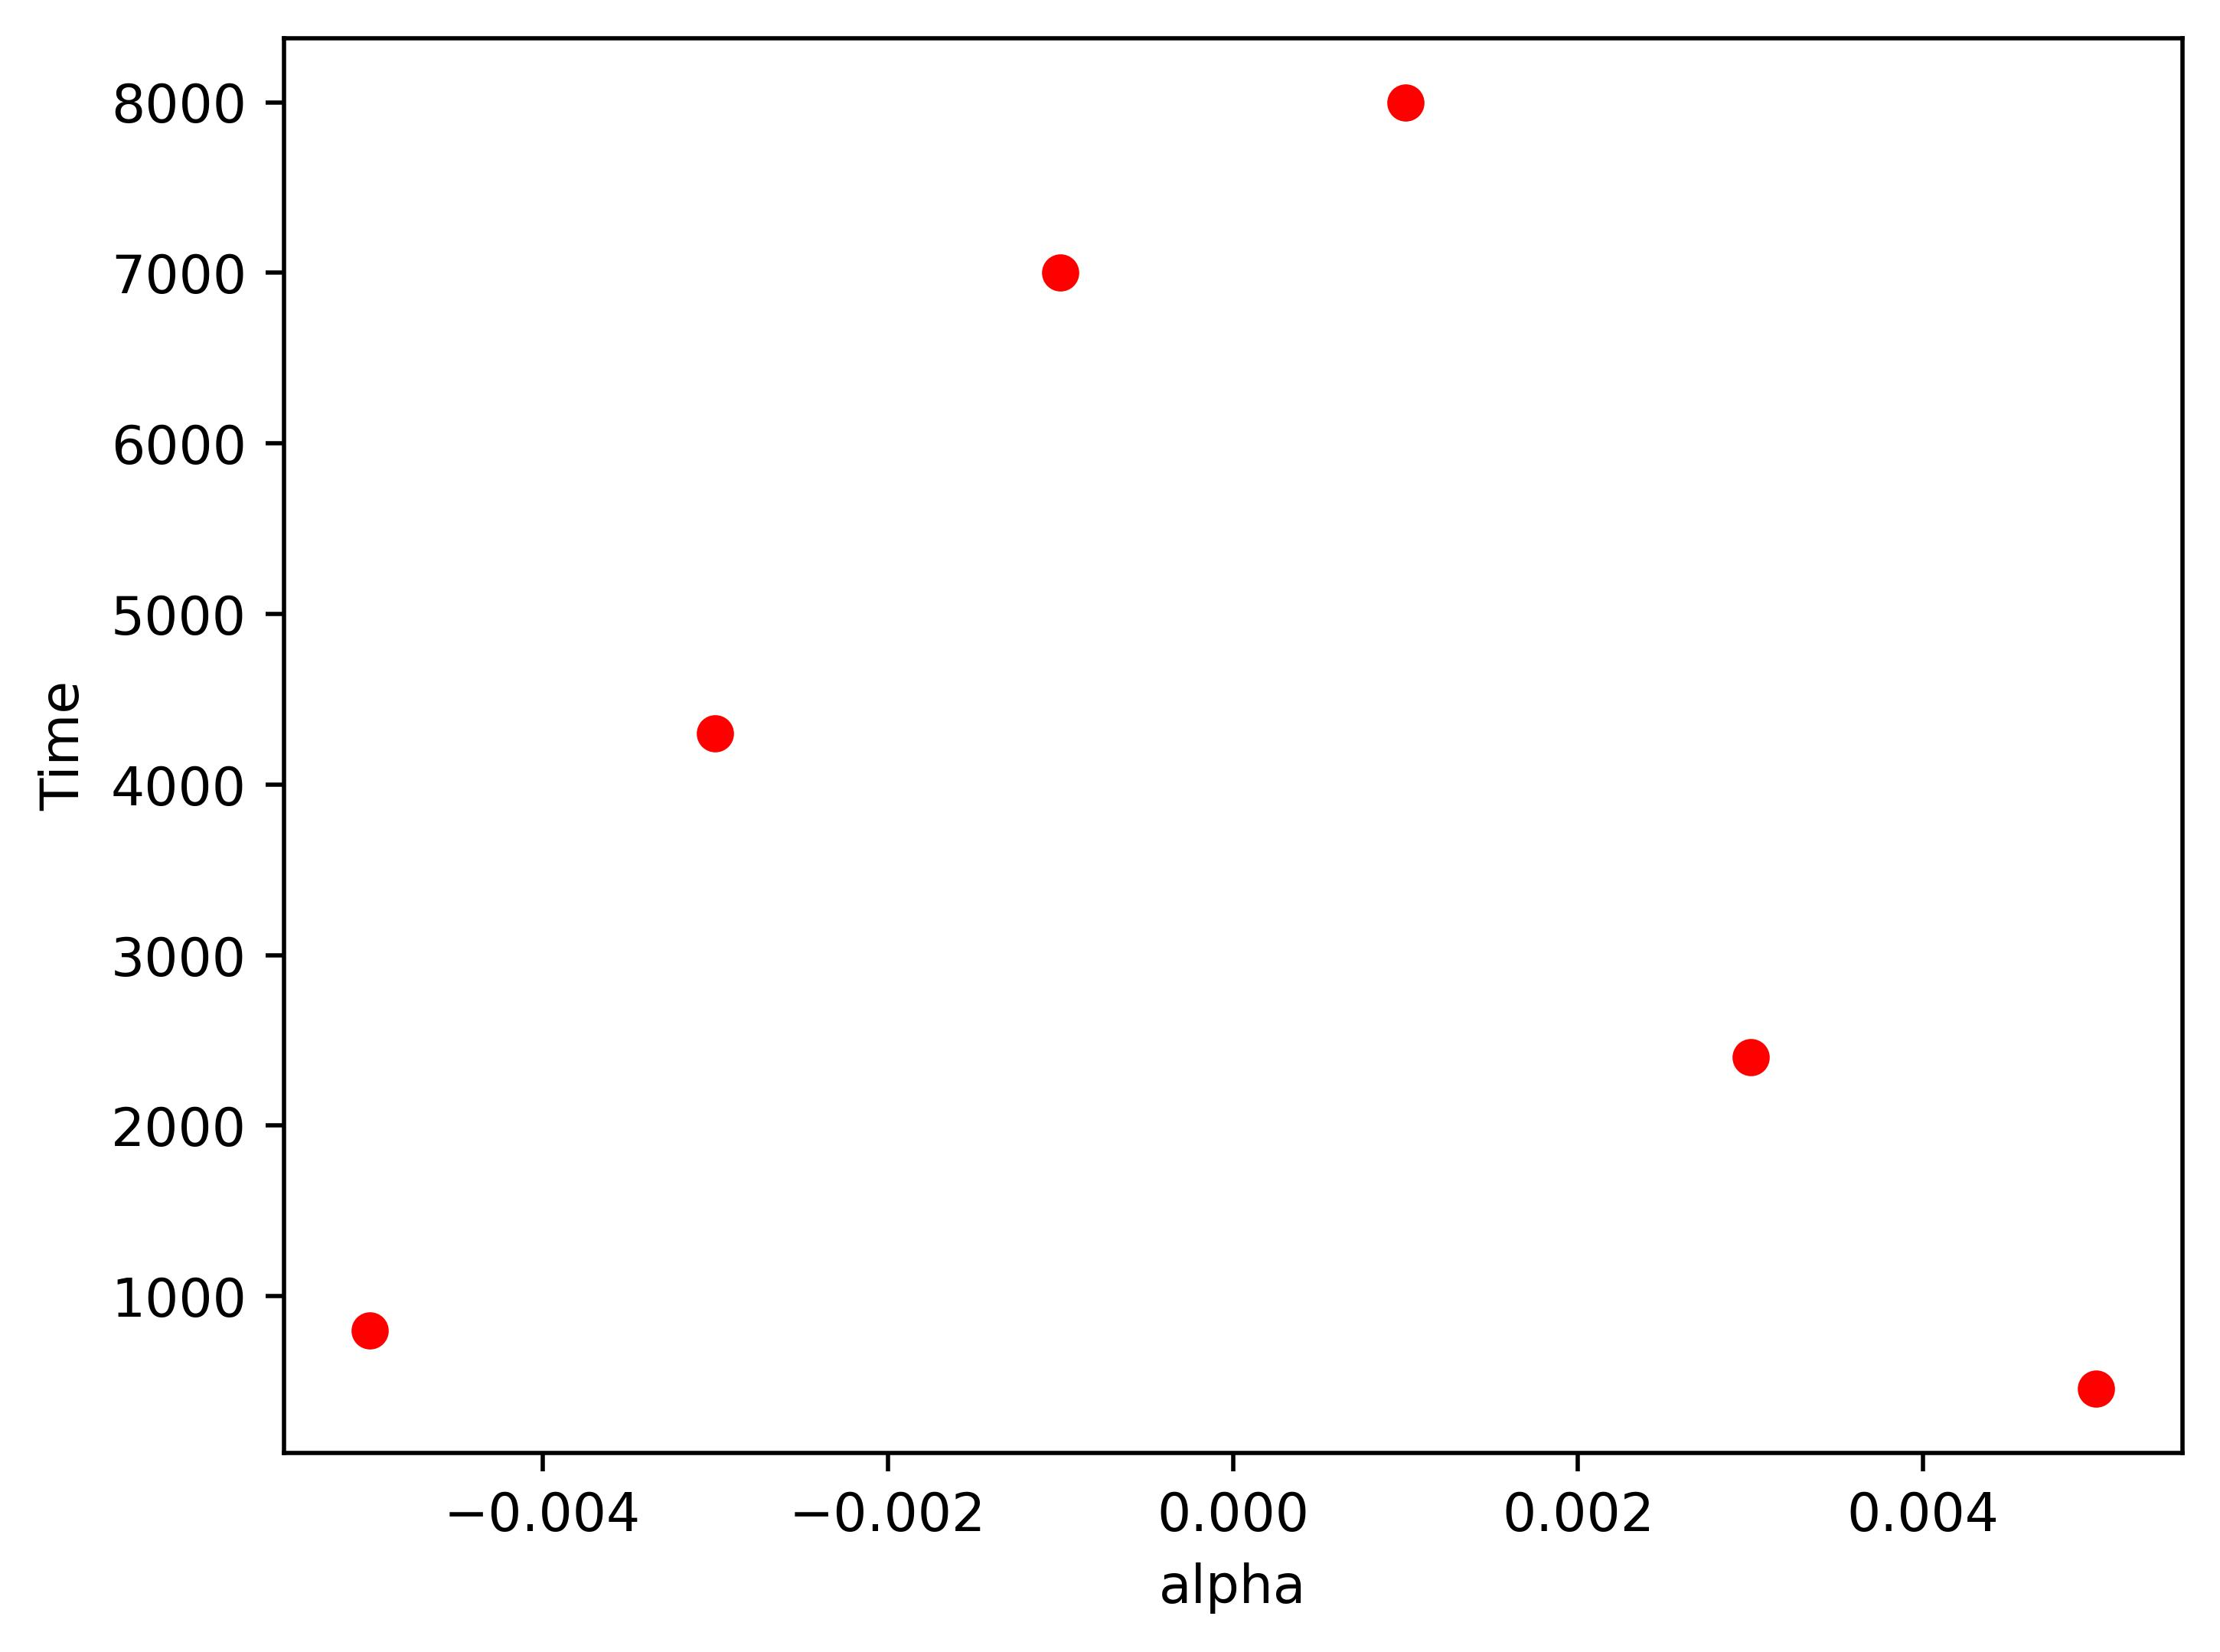
\includegraphics[width=0.4\textwidth]{SA2}
          \label{fig:Sensitivity_Analysis_2}
      }
\end{figure}
      

% 根据图\ref{fig:Model 1 sensitivity analysis}的结果,我们可以观察到在对参数 $\epsilon$ 进行扰动时,随着扰动项 $\epsilon$ 的增大,系统的最大稳定时间 $T_{max}$ 逐渐减少。这表明,随着扰动的增加,生态系统变得越来越脆弱,难以维持其稳定性。这种敏感性分析有助于我们了解生态系统对于外部扰动的响应。

% 另一方面,当对性转率 $\alpha$ 进行扰动时,我们观察到 $\alpha$ 的扰动比 $\epsilon$ 对 $T_{max}$ 的影响更为显著。这意味着七鳃鳗的性别比例机制对其生存环境的影响更为重要。这可能暗示着性别比例的变化对生态系统的稳定性产生了更大的影响,可能与繁殖和种群结构有关。

Based on the results shown in Figure \ref{fig:Sensitivity_Analysis_1}, \ref{fig:Sensitivity_Analysis_2} we observe that when perturbing the parameter $\epsilon$, the maximum stability time $T_{max}$ gradually decreases with the increasing perturbation of $\epsilon$. This indicates that, as the disturbance grows, the ecosystem becomes more fragile, making it challenging to maintain its stability. This sensitivity analysis helps us gain insights into the ecosystem's response to external disturbances.

On the other hand, when perturbing the mating rate $\alpha$, we observe that the impact of $\alpha$ on $T_{max}$ is more pronounced compared to the effect of $\epsilon$. This suggests that the gender ratio mechanism of the lamprey has a more significant influence on its survival environment. This may imply that changes in gender ratios have a greater impact on the stability of the ecosystem, possibly related to reproduction and population structure.

\section{Model Evaluation and Further Discussion}

\subsection{Strengths}
% 1.模型通过多学科综合方法,探讨了七鳃鳗性别比例变化的生态学机制,本文采用了Lotka-Vollerra慢型细胞自动机模型和寄生主寄生物动力学模型,从不同角度考察了性别比例变化的影响。这为生态保护和资源管理提供了重要参考,并为多学科综合方法研究七鳃鳗性别比例变化的生态学机制提供了里要参考。
% 2.模型结果与实际观察一致,具有较高的可信度。例如,Lotka-Volterra模型模拟结果显示,在资源匮乏环境下,七鳃鳗种群中雄性比例会明显增加,这与买际观察结果相一致。
%3.模型考虑了性别比例变化对生态系统的影响,具有代表性。例如,细胞自动机模型结果显示,性别比例变化有助于七鳃鳗适应环境,但也存在潜在的生态风险。
% 4.模型从不同角度考察了性别比例变化的影响,包括食物链、寄生关系等方面。例如,寄生主-寄生物动力学模型分析了性别比例变化对寄生关系的影响。

\begin{enumerate}
	\item The model explores the ecological mechanisms of gender ratio changes in lampreys through a multidisciplinary approach. This study employs the Lotka-Volterra slow-type cellular automaton model and a host-parasite dynamic model, examining the impacts of gender ratio changes from different perspectives. This provides crucial insights for ecological conservation and resource management, offering essential references for interdisciplinary studies on the ecological mechanisms of gender ratio changes in lampreys.

   \item The model results align with actual observations, demonstrating high credibility. For instance, the Lotka-Volterra model simulation results indicate a significant increase in the male proportion in lamprey populations under resource-scarce environments, consistent with empirical observations.

   \item The model takes into account the influence of gender ratio changes on the ecosystem, adding to its representativeness. For example, the cellular automaton model results suggest that gender ratio changes contribute to lampreys adapting to their environment but also pose potential ecological risks.

   \item The model investigates the impacts of gender ratio changes from various perspectives, including food chains and parasitic relationships. For instance, the host-parasite dynamic model analyzes the effects of gender ratio changes on parasitic relationships.
\end{enumerate}

\subsection{Weaknesses}
% 2.模型适用性有限,难以模拟复杂环境条件。例如,Lotka-Volterra模型假设环境条件恒定,这跟制了模型
% 的适用范围。
% 3.模型未考虑人类活动的影响,如捕捞和污染等。这可能会影模型结果的准确性
% 4.模型存在一定的复杂性,参数变化会对结果产生较大影响。例如,灵敏度分析结果显示,参数交化会导致模型结果产生较大波动。

\begin{enumerate}
	\item The model has limited applicability and struggles to simulate complex environmental conditions. For instance, the Lotka-Volterra model assumes constant environmental conditions, restricting the model's scope of application.

   \item The model does not consider the impact of human activities, such as fishing and pollution. This omission could potentially affect the accuracy of the model results.


      \item The model exhibits a certain level of complexity, and parameter variations can significantly influence the results. For example, sensitivity analysis results indicate that parameter interactions can lead to substantial fluctuations in model outcomes.
\end{enumerate}

\section{Conclusion}

\begin{enumerate}
\item For question one, studies have shown that changes in the sex ratio of lampreys can affect their predation efficiency. In particular, the significant increase in the male ratio in the lamprey population in resource-poor environments may lead to higher predation efficiency, thereby affecting the structure and function of the food chain. As a top predator, humans will also be affected by changes in the lamprey population. Furthermore, changes in the sex ratio may cause fluctuations in population size, affecting the stability of the ecosystem. While changes in the sex ratio can help lampreys adapt to environmental changes, such as resource-poor environments, this may also bring ecological risks. In terms of reproductive strategies, changes in the sex ratio can help lampreys optimize their reproductive strategies, such as finding suitable breeding environments and increasing the success rate of reproduction. However, this may also lead to a decline in the reproductive rate. 
%针对问题一,研究表明,七鳃鳗性别比例的变化会影响其捕食效率。特别是在资源匮乏的环境下,七鳃鳗种群中雄性比例显著增加,这可能提高捕食效率,从而影响食物链结构和功能。作为顶级捕食者,人类也会受七鳃鳗种群数量变化的影响。此外,性别比例的变化可能导致种群波动,影响生态系统稳定性。尽管性别比例变化有助于七鳃鳗适应环境变化,如资源匮乏环境,但这种变化也可能带来生态风险。在繁殖策略方面,性别比例变化有助于七鳃鳗优化繁殖策略,例如找到适宜的繁殖环境,提高繁殖成功率。然而,这也可能导致繁殖率下降。
\item For question two, according to the model results, we can find that the ability of lampreys to change their sex ratio has advantages in terms of adaptability and reproductive optimization. Specifically, in the Lotka-Volterra model, when resources are scarce, the male proportion in the lamprey population significantly increases, which may improve predation efficiency and thereby affect the structure and function of the food chain. In the cellular automaton model, the simulation results show that when the sex ratio remains constant, the lamprey population grows faster, but with greater resource consumption. In addition, the parasitism-host dynamics model also shows that as the number of lamprey infections increases, the lamprey population fights against the threat of parasites by increasing the male proportion. Although these model results show that the ability of lampreys to change their sex ratio has advantages in adaptability and reproductive optimization, it may also lead to some adverse effects. For example, changing the sex ratio may reduce overall reproductive rates, bring instability to the ecosystem, and reduce genetic diversity within the population.
%针对问题二,根据模型结果,我们可以发现七鳃鳗改变性别比例的能力在适应性和繁殖优化方面具有优势。具体来说,在Lotka-Volterra模型中,当资源稀缺时,七鳃鳗种群中雄性比例显著增加,这可能会提高捕食效率,进而影响食物链结构和功能。而在元胞自动机模型中,模拟结果显示,当性别比例保持不变时,七鳃鳗种群增长更快,但伴随着更大的资源消耗。此外,寄生-宿主动态模型也表明,随着七鳃鳗感染寄生虫数量的增加,七鳃鳗种群通过增加雄性比例来对抗寄生虫的威胁。虽然这些模型结果显示七鳃鳗改变性别比例的能力在适应性和繁殖优化方面具有优势,但它也可能导致一些不利影响。例如,改变性别比例可能降低整体繁殖率,对生态系统带来不稳定性,降低种群内的遗传多样性等。
\item For question three, according to the model results, we can find that the ability of lampreys to change their sex ratio has advantages in terms of adaptability and reproductive optimization. Specifically, in the Lotka-Volterra model, when resources are scarce, the male proportion in the lamprey population significantly increases, which may improve predation efficiency and thereby affect the structure and function of the food chain. In the cellular automaton model, the simulation results show that when the sex ratio remains constant, the lamprey population grows faster, but with greater resource consumption. In addition, the parasitism-host dynamics model also shows that as the number of lamprey infections increases, the lamprey population fights against the threat of parasites by increasing the male proportion. Although these model results show that the ability of lampreys to change their sex ratio has advantages in adaptability and reproductive optimization, it may also lead to some adverse effects. For example, changing the sex ratio may reduce overall reproductive rates, bring instability to the ecosystem, and reduce genetic diversity within the population.
%针对问题三,根据模型结果,我们可以发现七鳃鳗改变性别比例的能力在适应性和繁殖优化方面具有优势。具体来说,在Lotka-Volterra模型中,当资源稀缺时,七鳃鳗种群中雄性比例显著增加,这可能会提高捕食效率,进而影响食物链结构和功能。而在元胞自动机模型中,模拟结果显示,当性别比例保持不变时,七鳃鳗种群增长更快,但伴随着更大的资源消耗。此外,寄生-宿主动态模型也表明,随着七鳃鳗感染寄生虫数量的增加,七鳃鳗种群通过增加雄性比例来对抗寄生虫的威胁。虽然这些模型结果显示七鳃鳗改变性别比例的能力在适应性和繁殖优化方面具有优势,但它也可能导致一些不利影响。例如,改变性别比例可能降低整体繁殖率,对生态系统带来不稳定性,降低种群内的遗传多样性等
\item For question four, based on the model results, an ecosystem with a variable sex ratio in the lamprey population may offer advantages to other organisms in the ecosystem, such as parasites. Specifically, in the parasitism-host dynamics model, as the number of lamprey infections increases, the lamprey population fights against the threat of parasites by increasing the male proportion. This unique adaptive behavior allows the lamprey population to survive under the pressure of parasitic threats and maintain a relatively balanced ecosystem. The outcomes of this natural selection contribute to ensuring the coexistence of lamprey populations and parasites, mitigating the threat of extinction. 
%针对问题四,根据模型结果,一个拥有可变性别比例七鳃鳗种群的生态系统对其他生物如寄生虫可能具有优势。具体来说,在寄生-宿主动态模型中,随着七鳃鳗感染寄生虫数量的增加,七鳃鳗种群通过增加雄性比例来对抗寄生虫的威胁。这种独特的适应性行为使得七鳃鳗种群在寄生虫的威胁下得以生存,并维持一个相对平衡的生态系统。这种自然选择的结果有助于确保七鳃鳗种群与寄生虫的共存,减轻灭绝威胁。
\end{enumerate}



\bibliographystyle{plain}
\bibliography{reference}

% \begin{appendices}

% Here are simulation programmes we used in our model as follow.\

% Model 1 equation code:
% \lstinputlisting[language=Python]{./code/one.py}

% Model 2 equation code:
% \lstinputlisting[language=Python]{./code/two.py}

% Model 3 equation code:
% \lstinputlisting[language=Matlab]{./code/three.m}
% \end{appendices}


\AImatter

\begin{ReportAiUse}{9}
\bibitem{AI1}
OpenAI ChatGPT3\\
Query1: lampreys introduction\\
Output: Lampreys are a group of primitive, jawless fish belonging to the order Petromyzontiformes. They are characterized by their unique, eel-like appearance and have been in existence for hundreds of millions of years, making them one of the oldest living vertebrate groups. These fascinating creatures are found in various aquatic environments, including freshwater and coastal areas.

Here are some key features and aspects of lampreys:

1. **Anatomy:**
   - *Jawless Mouth:* One of the most distinctive features of lampreys is their jawless mouth, which is adapted for attaching to and feeding on the blood of other fish and sometimes other vertebrates. They use a rasping tongue filled with keratinized teeth to make a hole in the host's skin, and then they feed on blood and bodily fluids.

   - *Eel-Like Body:* Lampreys have a slender, elongated body with a cartilaginous skeleton. Their skin is smooth, lacking scales, and their coloration varies among species.

2. **Life Cycle:**
   - *Anadromous Migration:* Many lamprey species exhibit anadromous behavior, migrating between freshwater and the ocean. They spawn in freshwater, and the larvae (called ammocoetes) typically live in sediment, filter-feeding on organic particles.

   - *Metamorphosis:* Lampreys undergo a fascinating metamorphosis as they transition from the larval stage to adults. During this process, they develop the characteristic jawless mouth and transform into parasitic or non-parasitic adults, depending on the species.

3. **Habitat:**
   - Lampreys can be found in a variety of aquatic habitats, ranging from freshwater rivers and lakes to coastal areas and even the open ocean. They are known to migrate over long distances.

4. **Ecological Role:**
   - Lampreys play a role in ecosystems as both predators and prey. As parasitic adults, they may impact fish populations by feeding on their blood. At the same time, they serve as a food source for larger fish, birds, and mammals.

5. **Economic Significance:**
   - Some lamprey species are considered pests in fisheries as they can negatively impact economically important fish species. Efforts are made to control lamprey populations in certain regions to protect fish stocks.

6. **Conservation:**
   - Some lamprey species face conservation challenges due to habitat loss, pollution, and barriers to migration (such as dams). Conservation efforts are underway to better understand and protect these ancient and ecologically important fish.

Lampreys, with their unique life cycle and ecological role, continue to be a subject of scientific interest and research.

\bibitem{AI2}
OpenAl ChatGPT3\\
Query1: Introducing Cellular Automata\\
Output: Cellular Automata (CA) are computational models that consist of a grid of cells, each of which can be in one of a finite number of states. These models evolve over discrete time steps based on a set of rules governing the state transitions of cells, typically determined by the states of neighboring cells.

The basic components of a cellular automaton include:

1. **Grid**: A regular lattice of cells, usually arranged in one, two, or three dimensions.

2. **Cell States**: Each cell can be in one of a finite set of states. The states often represent different conditions, such as "alive" or "dead" in Conway's Game of Life, or various colors in other applications.

3. **Neighborhood**: The set of neighboring cells that influence the state of a given cell. The neighborhood can vary, including Moore neighborhood (all adjacent cells) or von Neumann neighborhood (only orthogonal cells).

4. **Rules**: The set of rules determines how the state of each cell evolves over time based on its current state and the states of its neighbors. These rules are typically expressed as a transition function.

Cellular Automata can exhibit a wide range of behaviors, from simple and predictable patterns to complex and seemingly chaotic dynamics. They have found applications in various fields, including physics, biology, computer science, and artificial life.

One of the most well-known examples of Cellular Automata is Conway's Game of Life, which operates on a two-dimensional grid of cells with simple rules:

1. Any live cell with fewer than two live neighbors dies (underpopulation).
2. Any live cell with two or three live neighbors survives.
3. Any live cell with more than three live neighbors dies (overpopulation).
4. Any dead cell with exactly three live neighbors becomes alive (reproduction).

The Game of Life produces fascinating and intricate patterns, and it has become a popular topic in computer science and recreational mathematics.

Cellular Automata offer a powerful way to model and explore emergent phenomena, and they have inspired research and discussions in the fields of complexity theory and artificial life.
\bibitem{AI3}
OpenAI ChatGPT3\\
Query1: Describe the Lotka-Volterra (LV) model\\
Output: The Lotka-Volterra (LV) model is a pair of differential equations that describe the dynamics of predator-prey interactions in ecological systems. It was independently developed by Alfred Lotka and Vito Volterra in the early 20th century.

The basic form of the Lotka-Volterra model consists of two equations, one for the prey population (usually denoted as "x") and one for the predator population (usually denoted as "y"). The model assumes the following:

1. **Prey Equation:**
   \[ \frac{dx}{dt} = \alpha x - \beta xy \]
   This equation represents the rate of change of the prey population (\(x\)). The term \(\alpha x\) represents the prey's intrinsic growth rate, and the term \(\beta xy\) represents the rate at which the prey is captured and consumed by the predators.

2. **Predator Equation:**
   \[ \frac{dy}{dt} = \delta xy - \gamma y \]
   This equation represents the rate of change of the predator population (\(y\)). The term \(\delta xy\) represents the rate at which predators increase their population by consuming prey, and \(\gamma y\) represents the death rate of predators.

In these equations, the parameters have the following meanings:
- \(\alpha\): Prey birth rate or intrinsic growth rate.
- \(\beta\): Rate at which prey is captured and consumed by predators.
- \(\delta\): Rate at which predators increase their population by consuming prey.
- \(\gamma\): Predator death rate.

The Lotka-Volterra model assumes certain simplifications and idealizations, such as constant parameters and a closed system. It provides insights into the oscillatory nature of predator-prey interactions, demonstrating how the populations of predators and prey can fluctuate over time, creating cyclical patterns. However, it's essential to note that the model has limitations and may not fully capture the complexity of real ecological systems. Extensions and modifications have been proposed to address some of these limitations.

\end{ReportAiUse}

\end{document}

